\chapter{Vakcinace pohledem matematických modelů}
\label{Ucinnost_ockovani}

\textit{Luděk Berec}
\vspace{15mm}

\section*{Úvod}

Očkování je spolu s nefarmaceutickými opatřeními a případnými léky jedním ze tří pilířů boje proti epidemiím. Zatímco při opakovaných epidemiích téže infekce je určitá část populace už imunizovaná (proděláním infekce či očkováním případnou vakcínou), při epidemiích nových patogenů, jako je virus SARS-CoV-2, je vakcína k dispozici nejdříve až po určité době od jejich vypuknutí. V tomto ohledu byl vývoj vakcín proti covid-19 nesmírně rychlý, byť nesmíme zapomínat, že zásadně stavěl na dlouholetém základním výzkumu \cite{Pardi_etal2018}. Distribuce vakcín proti covid-19 začala koncem roku 2020 a proti původním očekáváním nebyly jejich dodávky po nějakou dobu dostatečné. V současnosti se situace v Evropě výrazně zlepšila, avšak podobným problémům s nedostatkem vakcín jako Evropa před několika měsíci nyní čelí řada mimoevropských zemí.

Očkovací kampaň je složitý proces, který pro svůj efektivní průběh vyžaduje dobré plánování. Jako v řadě jiných aspektů epidemie, i zde se ukázala nezastupitelná role matematického modelování. První a snad tou nejdůležitější výzvou v tomto směru byla otázka, jakým způsobem omezený přísun vakcín mezi obyvatelstvo distribuovat a jaké skupiny společnosti upřednostnit \cite{Bubar_etal2021,Moore_etal2021b}. Jednou z prioritních skupin se z pochopitelných důvodů stali zdravotníci a další profese nutné pro zajištění nezbytné zdravotní péče, a to nejen o pacienty s covid-19. Pro prioritizaci mezi ostatními pak bylo nezbytné stanovit optimalizační kritérium, tedy čeho chceme vakcinací prioritně dosáhnout. Nabízí se možnost minimalizovat celkový počet zemřelých, ztracené roky života nebo celkové počty nakažených. Zatímco v případě prvních dvou kritérií se shodně ukázalo jako optimální nejdříve očkovat nejstarší věkové skupiny a následně postupovat k mladším ročníkům, v případě minimalizace celkového počtu nakažených se ukázali být prioritní skupinou lidé středního věku, neboť v rámci této skupiny dochází k největšímu počtu kontaktů, a je v ní tedy nejvyšší prevalence \cite{Bubar_etal2021,Moore_etal2021b}. Zdá se, že všude na světě zvítězil etický přístup a s očkováním se postupuje od nejstarších k nejmladším ročníkům.

Druhou otázkou, která se objevila v reakci na nedostatečné dodávky vakcín, bylo, jak i při tomto omezeném přísunu zvýšit rychlost očkování. Diskuse se brzy stočila k tomu, zda a jak zvýšit časový rozestup mezi dávkami u dvoudávkových vakcín, což jsou zatím všechny vakcíny kromě látky Janssen společnosti Johnson \& Johnson. Základní myšlenka za případným zvýšením doby mezi dávkami ve srovnání s rozestupy doporučenými výrobci je tato: místo toho, abychom za každou vyočkovanou první dávku odložili vždy jednu další dávku stranou, můžeme díky odložení druhé dávky aktuálně naočkovat mnohem více lidí, což při dostatečné účinnosti vakcín už po první dávce může mít na další šíření patogenu výraznější pozitivní dopad \cite{Paltiel_etal2021,Tuite_etal2021}\footnote{Tento argument se nyní může zdát nesprávný v souvislosti s virovou variantou delta, neboť účinnost vakcín po první dávce je proti této variantě velmi nízká \cite{delta}. Naše výsledky, které představíme dále v textu, však tuto variantu pokrývají.}. Není to však tak jednoduché, jak by se na první pohled mohlo zdát, neboť zvýšení počtu prvních dávek nyní znamená zpomalení rychlosti očkování první dávkou později, protože se pak budou muset ve velké míře aplikovat druhé dávky. Dopady jakékoli strategie odkladu druhé dávky tak mohou záviset a velmi pravděpodobně závisejí na řadě faktorů včetně rychlosti dodávek vakcín, aktuální intenzity epidemie, ale také toho, jak vakcína funguje (kterou část cesty od nakažení po uzdravení nejvíce ovlivňuje). 

V této kapitole si nejprve řekneme něco z historie matematického modelování očkování, které mimo jiné dalo světu myšlenku kolektivní imunity, podíváme se na některé typy očkování a přístupy k jejich modelování a nakonec si představíme výsledky studie, kterou jsme v centru BISOP provedli za účelem posouzení výhodnosti delšího rozestupu mezi dvěma dávkami vakcíny.

\section*{Něco z historie matematického modelování vakcinace}

Zřejmě první matematický model infekční nemoci, který zahrnoval vakcinaci, je nejspíše zároveň i prvním matematickým modelem infekční nemoci vůbec. Autorem tohoto modelu, který jsme si podrobněji představili v kapitole \ref{Typy_modelu}, je švýcarský lékař, fyziolog, matematik, fyzik a biolog Daniel Bernoulli (1700--1782). Šlo o tzv. variolaci, metodu, která spočívala v přenesení rozdrceného stroupku nebo tekutiny z puchýřku člověka nakaženého lehčí formou neštovic do kůže zdravého člověka s tím, že se u takového člověka vytvoří ochrana proti těžší formě infekce. Bernoulli se pokusil určit, zda dlouhodobé přínosy variolace převáží nad okamžitými riziky. Na základě dobových dat o populační struktuře spočítal, že zatímco očekávaná délka života v populaci s pravými neštovicemi je 26 let a 7 měsíců, očekávaná délka života v populaci bez pravých neštovic je 29 let a 8 měsíců \cite{Bacaer2011}. Následně odhadl, že variolace má z hlediska přínosu pro společnost smysl, pokud je pravděpodobnost úmrtí po variolaci nižší než $0.11$. Reálně docházelo k úmrtím pouze přibližně v 1\,\% případů. Přestože na pravé neštovice zemřela i řada významných osobností té doby, nezískala variolace v Evropě přílišnou podporu \cite{Bacaer2011}.

V kapitole \ref{Typy_modelu} jsme si též představili tzv.\ SIR model epidemie vyvinutý A. G. McKendrickem a W. O. Kermackem, pány, kteří položili základy obecné teorie epidemií, jak ji známe dnes. Z tohoto modelu lze snadno spočítat, že počty nových případů v populaci čítající $N$ jedinců začnou klesat, jakmile podíl imunizovaných jedinců v populaci, tedy jedinců aktuálně infekčních ($I$), už uzdravených ($R$) a naočkovaných ($V$), bude větší než určitá kritická hodnota $K$ daná základním reprodukčním číslem $R_0$:
\begin{equation}
\frac{I+R+V}{N} > K = 1-\frac{1}{R_0}.
\end{equation}
Tento výpočet je založen na předpokladu 100\% účinnosti vakcíny z hlediska zabránění infekci a předpokladu, že získaná imunita je trvalá. V případě nemoci covid-19 je rozsah publikovaných odhadů základního reprodukčního čísla poměrně velký, zhruba $R_0 = 2-6$, ale můžeme najít i menší či větší hodnoty \cite[a uvnitř citované reference]{Billah_etal2020,Locatelli_etal2021}. Pro \emph{práh kolektivní imunity} by tak platilo $K = 0.5-0.83$, tedy imunizace $50--83\,\%$ populace by měla zabránit systematickému růstu počtu nových případů (avšak z kapitoly \ref{Typy_modelu} už víme, že SIR model je pro covid-19 přílišným zjednodušením). Při dosažení hodnoty $K$ mluvíme o dosažení tzv. \emph{kolektivní imunity}, kdy už v zásadě není možné, aby počet nově nakažených v populaci systematicky rostl. Pro potlačení epidemie tedy není nutné, aby se nakazili či naočkovali všichni (někteří z nás se z různých důvodů očkovat ani nemohou), protože jsou imunizovaným kolektivem chráněni (z populačního hlediska) i ti neimunizovaní. Každá vakcína je však nedokonalá jak co do účinnosti, tak co to trvání imunizace, a je proto nutné uvažovat o komplikovanějších modelech a vyšších hodnotách $K$ \cite{K1,K2}.

V případě opakovaných epidemií téže infekce může být kolektivní imunity dosaženo i v meziepidemickém období, což ve své podstatě zabrání vypuknutí jakékoli další epidemie takové infekce. Infekcí, u které se podařilo pomocí očkování dosáhnout globální kolektivní imunity, jsou pravé neštovice \cite{smallpox1}. Už v první polovině 20.\ století se podařilo díky očkování zbavit pravých neštovic Evropu a Spojené státy. Kritické pro celosvětové vyhubení tak bylo zvládnout situaci také v Africe, Asii a Jižní Americe. A právě na tyto oblasti se primárně zaměřilo WHO v jedinečné globální kampani, která měla za cíl právě dosažení kolektivní imunity. Tuto kampaň jako ředitel sekce infekčních nemocí spoluorganizoval i český epidemiolog Karel Raška (1909--1987) \cite{smallpox2}. Základem této kampaně bylo tzv. prstencové očkování, kdy se očkovalo zejména kolem ohnisek nákazy. Důležitá byla také striktní izolace nakažených a rozsáhlá osvětová kampaň.

Řadu dětských nemocí (např.\ dětskou obrnu, záškrt, spalničky) se podařilo eradikovat lokálně. V roce 2020 se celosvětově nakazilo dětskou obrnou něco málo přes 1000 osob, z nichž jen 140 divokou variantou viru. Jedinými dvěma zeměmi, kde byla tato infekce klasifikována jako endemická, byly Pákistán a Afghánistán. Cíl dosažení kolektivní imunity u dětských nemocí má však dva silné protihráče: vysoké základní reprodukční číslo, a tedy vysoký práh kolektivní imunity, a také nesnadnost v zemích třetího světa naočkovat dostatečný počet novorozených dětí dostatečně rychle. V průběhu času byly zformulovány tři hlavní indikátory pro možnost úspěšné eradikace patogenu \cite{Dowdle1999}: (i) existuje účinný nástroj pro přerušení přenosu infekce (zde hraje dominantní roli vakcinace), (ii) existují účinné diagnostické nástroje k detekci nakažených (za účelem jejich efektivní izolace a trasování kontaktů), (iii) lidé jsou pro daný patogen nezbytnými hostiteli (tedy neexistuje jiný rezervoár patogenu v prostředí). A všechno tohle dobře fungovalo u pravých neštovic.

Pro ilustraci dopadů očkování na epidemie uvažujme SIR model, do kterého doplníme proces očkování. Nechť $\theta$ je rychlost očkování (tedy počet lidí naočkovaných např. za jeden den) konstantní, vakcína je 100\% účinná a získaná imunita je trvalá. Nechť je dále vakcína k dispozici až po určitém čase $T$ po vypuknutí epidemie. Možný model pak je
\begin{equation}
\begin{array}{l}
%\min\left\{S[t] - \beta \, \frac{S[t]\,I[t]}{N[t]}, \theta\right\}
\displaystyle{S[t+1] = S[t] - \beta \, \frac{S[t]\,I[t]}{N} - \theta}, \\[3ex]
\displaystyle{I[t+1] = I[t] + \beta \, \frac{S[t]\,I[t]}{N} - \gamma I[t]}, \\[3ex]
\displaystyle{R[t+1] = R[t] + \gamma I[t] + \theta},
\end{array}
\label{modSIRV}
\end{equation}
kde člen $\theta$ začne být „aktivní“ až v čase $T$ od vypuknutí epidemie (pokud je $\theta$ větší než aktuální počet vnímavých jedinců $S[t]$ v populaci, naočkujeme všechny zbývající vnímavé jedince a jejich počet tak klesne na nulu). Závislost časového průběhu počtu nově nakažených (tzv.\ \emph{incidenci}), $\beta S[t] I[t]/N$, pro různé hodnoty $\theta$ a $T$ ilustruje obr.\,\ref{SIRvacc}.

\begin{figure}[h]
	\begin{center}
		\begin{minipage}[m]{0.45\linewidth}
			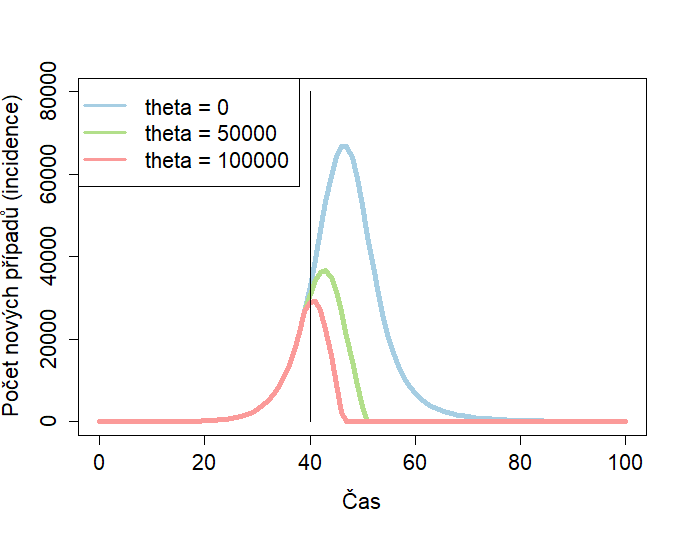
\includegraphics[width=0.99\textwidth]{pic/epidemicSIRvacc1.png}
		\end{minipage}
		\hspace{2ex}
		\begin{minipage}[m]{0.45\linewidth}
			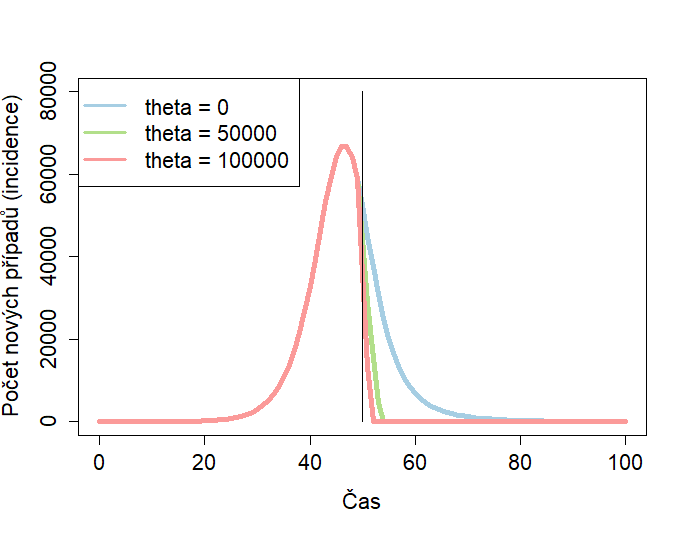
\includegraphics[width=0.99\textwidth]{pic/epidemicSIRvacc2.png}
		\end{minipage}
	\end{center}
	\caption{Závislost průběhu počtu nově nakažených v modelu (\ref{modSIRV}), $\beta \, S[t]\,I[t]/N$, pro různé hodnoty denního počtu naočkovaných vnímavých jedinců $\theta$ a začátku očkování $T$ (vyznačeno svislou čarou); $N=1000000$, $\beta=0.4$, $\gamma=0.1$.}
	\label{SIRvacc}
\end{figure}

Všechny země dnes rutinně očkují malé děti proti řadě jinak běžných dětských nemocí, v Česku například vakcínou Priorix proti spalničkám, zarděnkám a příušnicím a tzv. hexavakcínou proti záškrtu, tetanu, černému kašli, dětské obrně, žloutence typu B a onemocnění vyvolanému bakterií \emph{Haemaphilus influenzae} typu B. Jak ukazuje obr.\,\ref{measles1}, očkování proti spalničkám vedlo v Česku podobně jako v mnoha jiných zemích k podstatnému snížení nově doložených případů této infekce.

\begin{figure}[h]
	\begin{center}
		\begin{minipage}[m]{0.45\linewidth}
			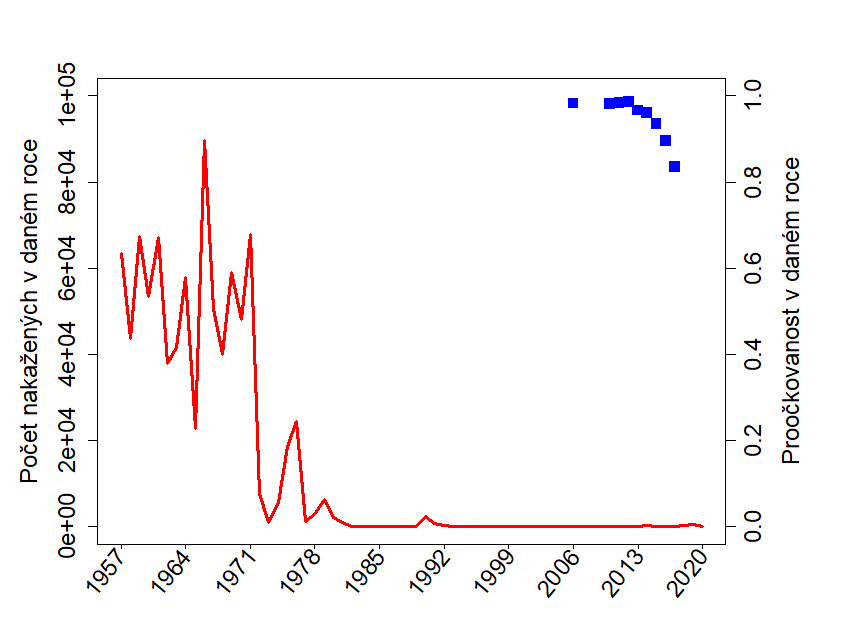
\includegraphics[width=0.99\textwidth]{pic/measles_data.png}
		\end{minipage}
		\hspace{2ex}
		\begin{minipage}[m]{0.45\linewidth}
			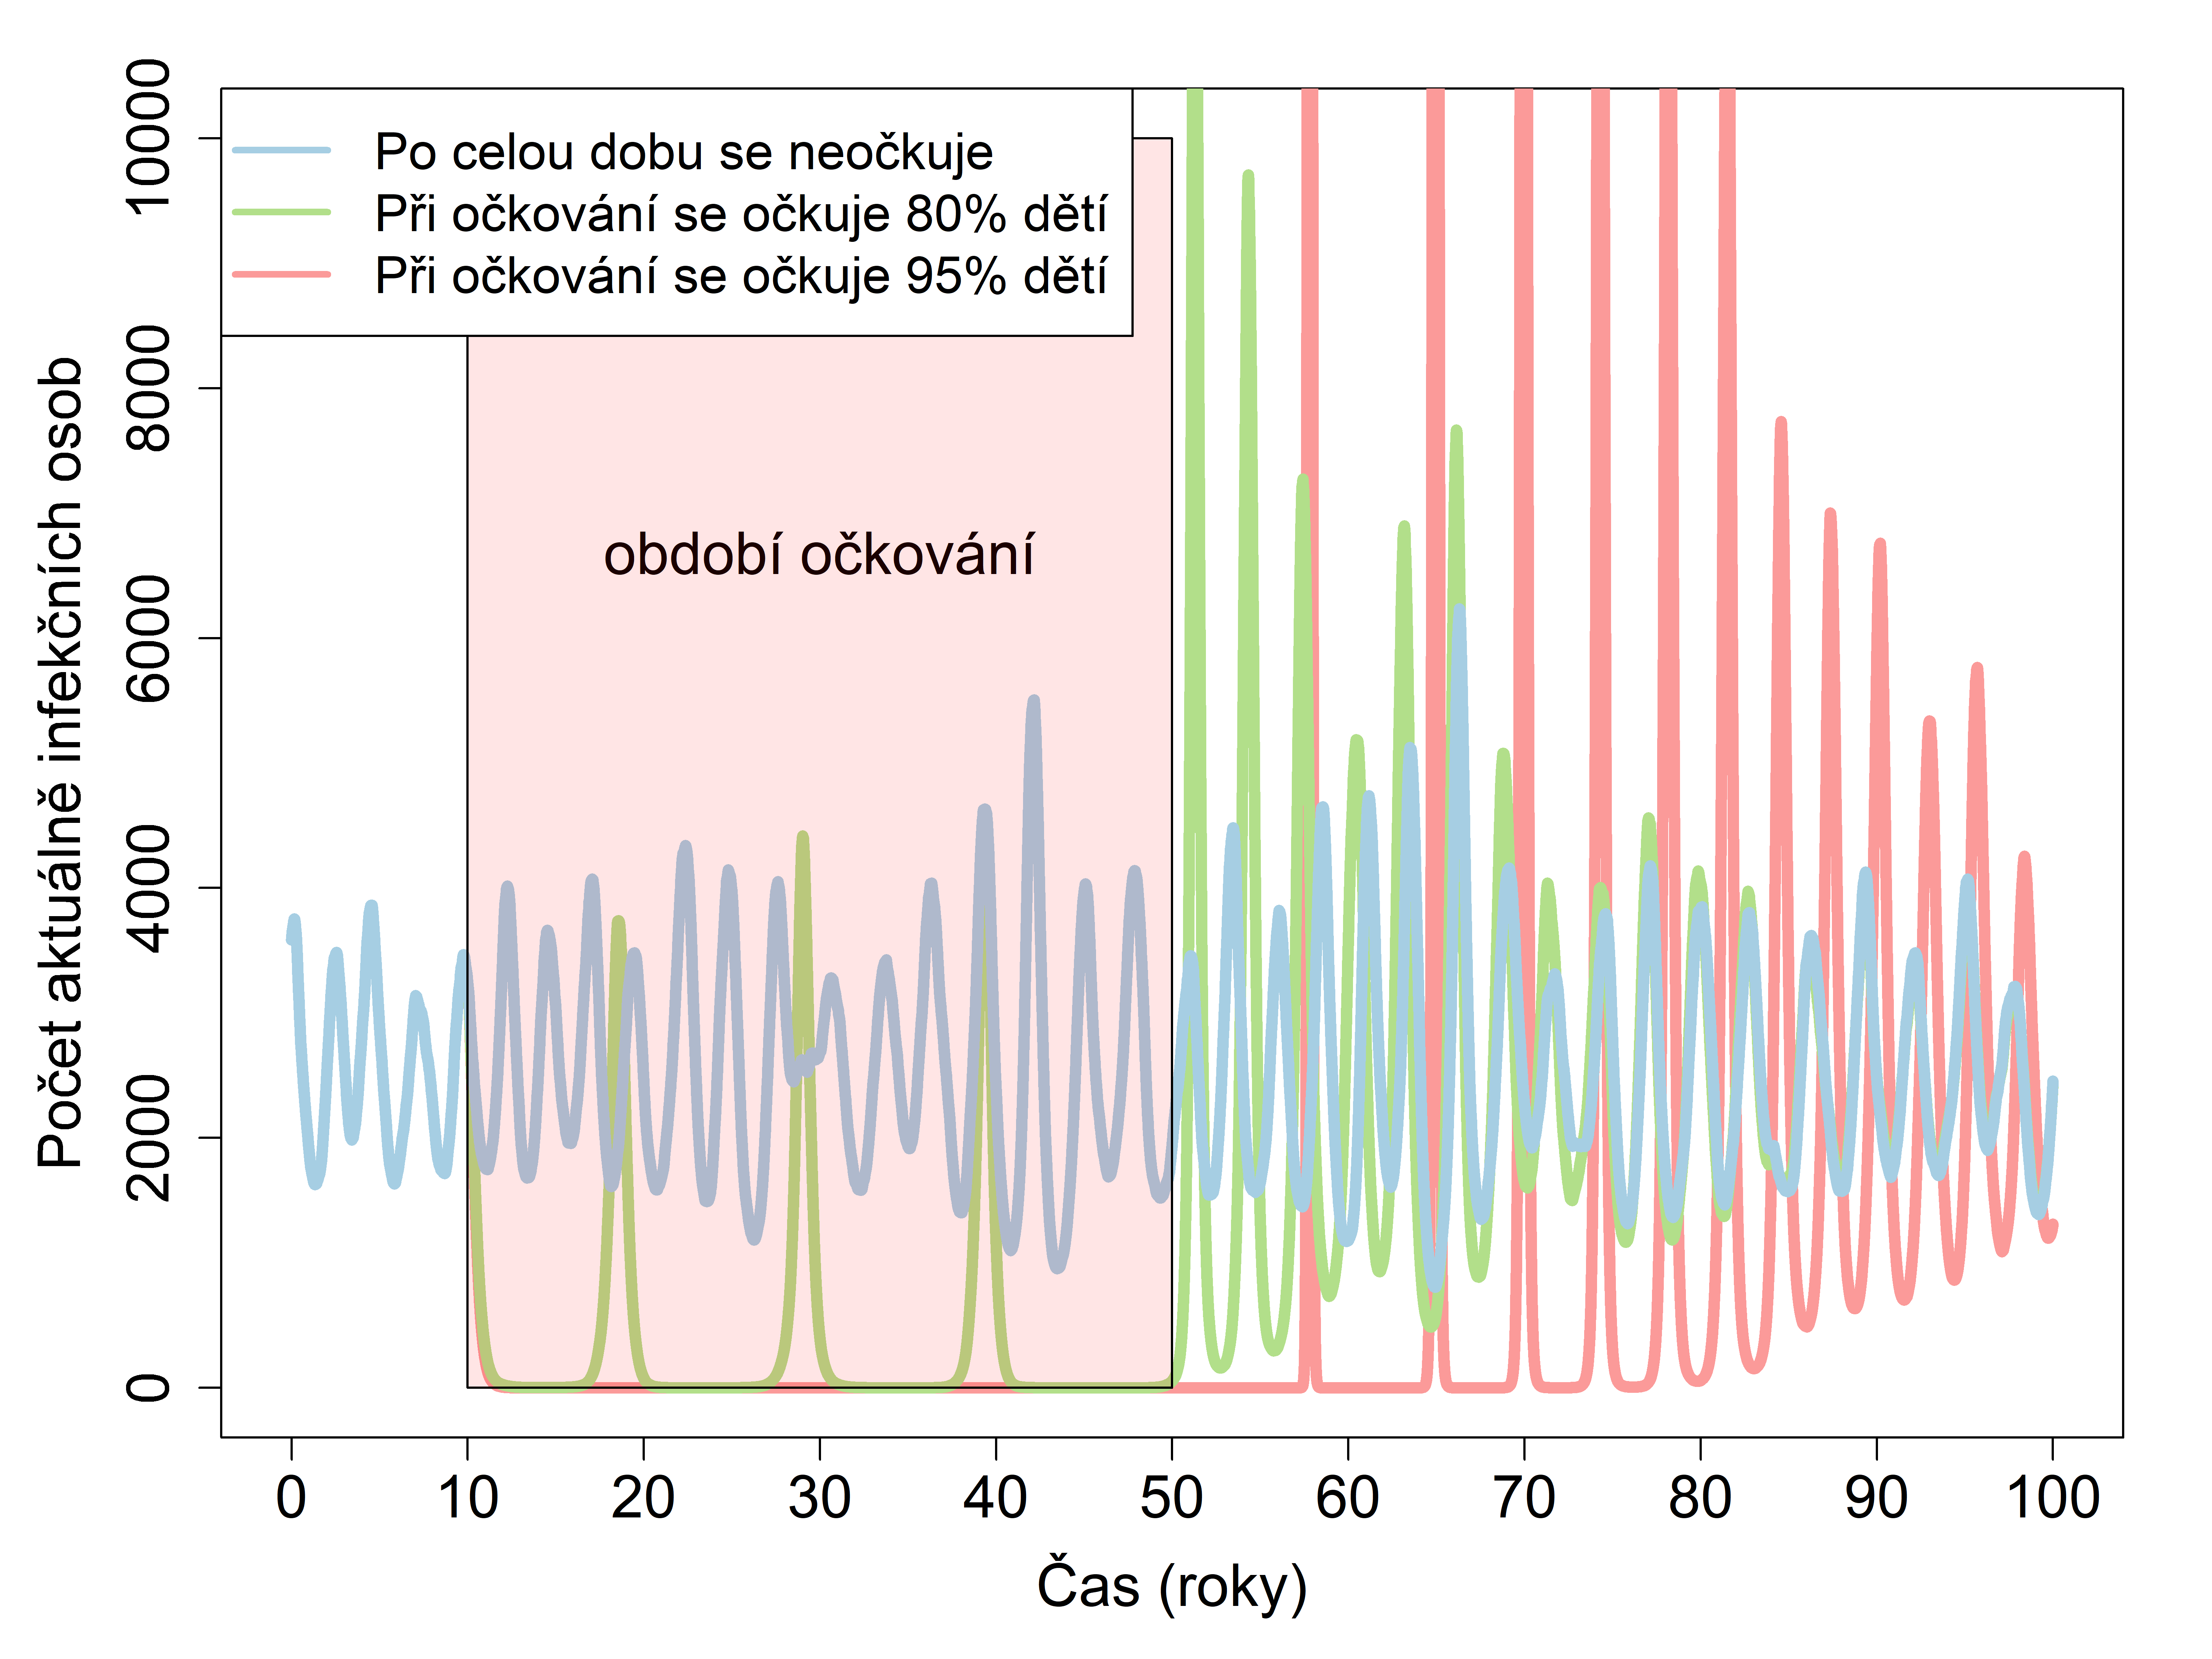
\includegraphics[width=0.99\textwidth]{pic/spalnicky2.png}
		\end{minipage}
	\end{center}
	\caption{Časová dynamika spalniček v Česku. Levý panel: průběh nově doložených případů spalniček v letech 1955--2018 (Zdroj: Státní zdravotní ústav). Pravý panel: Modelová dynamika spalniček bez očkování a se dvěma úrovněmi pokrytí populace očkováním v~modelu (\ref{measles-model1}), doplněném o sezonní a náhodné vlivy \cite{KeelingRohani2008}; $R_0=17$, $\gamma=1/7$, což odpovídá $\beta=2.43$, $\sigma=1/8$, $b=d=1/(70\times365)$. V pravém panelu je také zobrazena situace, kdyby se náhle proti spalničkám přestalo očkovat.}
	\label{measles1}
\end{figure}

Kandidátem na získání globální kolektivní imunity očkováním dlouho byly spalničky, nemoc, která stále po celém světě zabíjí stovky tisíc dětí ročně. Základní reprodukční číslo $R_0$ spalniček je často uváděno v rozsahu $12--18$, ale zřejmě může dosahovat i mnohem vyšších hodnot \cite{Guerra_etal2017}. Protože jde o endemickou (tedy trvale přítomnou) nemoc, potřebujeme k posouzení vlivu očkování modely, které uvažují populační demografii a nejlépe také rozlišují věkovou strukturu obyvatelstva. Ilustrujme si účinky dlouhodobé vakcinační strategie na pravděpodobně nejjednodušším modelu spalniček. Jde vlastně opět o SEIR model, který jsme si představili v kapitole \ref{Typy_modelu}, nicméně nyní je v něm třeba udělat dvě úpravy: zahrnout demografii populace (narození a přirozená úmrtí) a uvažovat vliv vakcinace v rámci členu popisujícího narození. Model pak vypadá takto \cite{BolkerGrenfell1993}:
\begin{equation}
	\begin{array}{l}
		\displaystyle{S[t+1] = S[t] + b (1-\nu) S[t] - \beta[t] \, \frac{S[t]\,I[t]}{N} - d S[t]}, \\[3ex]
		\displaystyle{E[t+1] = E[t] + \beta[t] \, \frac{S[t]\,I[t]}{N} - \sigma E[t] - d E[t]}, \\[3ex]
		\displaystyle{I[t+1] = I[t] + \sigma E[t] - \gamma I[t] - d I[t]}, \\[3ex]
		\displaystyle{R[t+1] = R[t] + b \nu S[t] + \gamma I[t] - d R[t]},
	\end{array}
	\label{measles-model1}
\end{equation}
kde $b$ je rychlost rozmnožování na jedince a $d$ je pravděpodobnost úmrtí jedince v daném časovém kroku. Často se předpokládá $b=d$, což znamená konstantní velikost populace (stačí všechny rovnice sečíst a vidíme, že celková populace, tedy $S+I+E+R$, v čase $t+1$ je stejná jako v čase $t$). I pro tento model platí, že práh kolektivní imunity je roven $1-1/R_0$, odpovídá tedy přinejmenším 92--95\% imunizaci společnosti. Během let 2010 až 2017 proočkovanost dětí v Česku postupně klesala z 98\,\% na 83\,\% \cite{spavac}. V roce 2019 dokonce WHO vyřadila Českou republiku kvůli rostoucímu počtu případů spalniček ze seznamu zemí, v nichž byla tato nemoc vymýcena \cite{spaend}. Podobné nárůsty lze pozorovat i jinde v Evropě \cite{Thornton2019}. Roste také výskyt například černého kašle \cite{Lavine_etal2011}. 

Dynamiku spalniček predikovanou modelem (\ref{measles-model1}) ukazuje obr.\,\ref{measles1}. Kromě stavu, kdy by se vůbec neočkovalo, uvádíme scénáře, kdy očkování pokrývá 80\,\% a 95\,\% nově narozených dětí. I tento velmi jednoduchý model předpovídá výraznou redukci infikovaných jedinců po zavedení očkování a scénář s 95\% pokrytím kvalitativně odpovídá pozorováním (obr.\,\ref{measles1}). Cyklická dynamika spalniček (ale i jiných dětských nemocí) je dána střídáním období, kdy infekce způsobí rychlý růst nakažených, reprodukční číslo klesne pod hodnotu 1 a množství infekčních jedinců začne naopak rychle klesat (určitá forma epidemie), a období, kdy nové děti znamenají postupně rostoucí skupinu vnímavých jedinců, která díky své velikosti v určité chvíli způsobí nárůst reprodukčního čísla nad hodnotu 1. V modelu (\ref{measles-model1}) jsou tyto oscilace postupně tlumeny \cite{KeelingRohani2008}. Pokud však tento model obohatíme o sezonní složku, typickou pro dětské infekce, a náhodné vlivy, výsledkem jsou přetrvávající a nepravidelné oscilace, jak je zachycuje obr.\,\ref{measles1} \cite{KeelingRohani2008}. 

Nabízí se otázka, co by se stalo, kdyby se s očkováním například proti spalničkám náhle přestalo. Takovou situaci ilustruje pravý panel v obr.\,\ref{measles1}. Kdyby se náhle s očkováním přestalo, po čase by se situace vrátila do doby před 70 a více lety (s přihlédnutím k současné vyšší délce života a nižší porodnosti než tenkrát), avšak ne okamžitě. Počty nemocných by zpočátku mnohem více oscilovaly, přičemž vyšší oscilace bychom pozorovali v situacích, kdy je procento proočkované populace vyšší. Důvodem je vyšší nárůst vnímavých jedinců po skončení očkování u proočkovanější populace. 

%\begin{figure}[h]
%	\begin{center}
%		%\includegraphics[width=0.6\textwidth]{measles_model2.png}
%	\end{center}
%	\caption{Časová dynamika spalniček v Česku v hypotetickém případě náhlého ukončení očkování, určená modelem (\ref{measles-model1}) doplněným o sezonní a náhodné vlivy \cite{KeelingRohani2008}; $R_0=17$, $\gamma=1/7$, což odpovídá $\beta=2.43$, $\sigma=1/8$, $b=d=1/(70\times365)$.}
%	\label{measles2}
%\end{figure}

Pro realistický popis dlouhodobé dynamiky dětských infekcí se používají věkově strukturované verze SEIR modelů, respektující věkové složení populace v dané zemi, stárnutí populace a počty efektivních kontaktů mezi jedinci stejných i různých věkových skupin \cite{KeelingRohani2008,VynnyckyWhite2010}.

\section*{Modelování vlivu očkování na covid-19}

Díky věkově specifickým efektům nemoci covid-19 (např.\ asymptomatičnost, pravděpodobnost hospitalizace, mortalita) jsou věkové rozrůznění a odpovídající kontaktní struktura zásadními elementy většiny skutečně prediktivních modelů covid-19 \cite[a mnoho dalších]{Davies_etal2020,Bubar_etal2021,Moore_etal2021,Rozhnova_etal2021}. Stejně tak je tomu i v naší studii dopadů očkování na covid-19 v Česku, kterou krátce popíšeme níže. O modelech, jejichž cílem bylo stanovit postup prioritizace očkování ve společnosti, jsme se již krátce zmínili v úvodu \cite{Bubar_etal2021,Moore_etal2021b}. Zmínili jsme také otázku možnosti zvýšení rozestupů mezi dvěma vakcinačními dávkami. Tato otázka byla aktuální i v Česku: do 1.\ dubna 2021 se očkovalo podle schémat doporučených výrobci (21 dní pro vakcínu Comirnaty společností Pfizer a BioNTech a 28 dní pro látku společnosti Moderna \cite{original_delay}), od tohoto data se pak doba do podání druhé dávky u obou vakcín zvýšila na šest týdnů \cite{new_delay}.

Existující modely, které otázku odkladu dávek řeší, jsou příliš jednoduché na to, aby poskytly robustní odpověď. Buď vůbec nezohledňují epidemickou dynamiku \cite{Tuite_etal2021}, nebo omezují možné strategie na výběr mezi dvěma dávkami s odkladem podle výrobce a jednou dávkou při naočkování dvojnásobného počtu osob \cite{Paltiel_etal2021}. Žádná z těchto studií tak nepopisuje současný stav epidemie ani nějaký více či méně realistický scénář distribuce dávek, respektující možné hodnoty mezidávkové periody. Proto jsme v centru BISOP vyvinuli modely, které by obě tyto charakteristiky zahrnovaly. Inspirováni nejčastěji podávanou vakcínou u nás, vakcínou Comirnaty společností Pfizer a BioNTech, uvažovali jsme mezidávkový interval 21 nebo 42 dní. Možnou výhodu posunutí druhé dávky jsme kvantifikovali jako rozdíl mezi počtem zemřelých k 30.\ červnu 2021 při rozestupu 42 dní a při rozestupu 21 dní, přičemž záporné hodnoty této statistiky znamenají méně mrtvých při rozestupu 42 dní. Pro nastavení modelu na současnou situaci jsme pochopitelně uvažovali průběh epidemie covid-19 v Česku, postupný nárůst a výslednou dominanci varianty alfa (dříve B.1.1.7) viru SARS-CoV-2 během ledna a února 2021, a také realistický scénář skutečné či plánované distribuce vakcín v Česku, včetně přijatého prioritizačního scénáře. 

Tři různé modely, které jsme pro hledání odpovědi na otázku výhodnosti odkladu druhé dávky vakcíny o 42 dní použili, jsou typu SEPIAR popsaného v kapitole \ref{Typy_modelu}. Ve všech jsme tak uvažovali asymptomatické infekční jedince, ať už po celou dobu infekce nebo jen po několik dní předcházejících objevení se symptomů. Zatímco jeden z modelů (model M) neuvažuje dynamiku hospitalizací, model F uvažuje hospitalizované jedince jako jednu agregovanou modelovou třídu. Model H, hlavní model v této studii, popisuje dynamiku v nemocnicích detailně, včetně přechodů mezi běžným lůžkem a jednotkou intenzivní péče, s dobami trvání jednotlivých stavů odhadnutými z dat poskytnutých Ústavem zdravotnických informací a statistiky ČR. Mezi modely je řada rozdílů také v jiných než hospitalizačních procesech. Všechny tři modely však rozlišují věkovou strukturu populace a různé typy kontaktů mezi jedinci. Modely M, F a H jsou detailně popsány v referencích \cite{M-techrep2021}, \cite{Smid2021seir} a \cite{vaccpaper}. Zde si představíme několik výsledků naší analýzy, další je pak možno najít v práci \cite{vaccpaper}, kde otázku možné výhodnosti odkladu druhé dávky vakcíny o 42 dní podrobně zkoumáme. 

Pro výchozí nastavení jsme každý model kalibrovali na aktuální průběh epidemie covid-19 a vývoj očkování v Česku. Protože jsme model kalibrovali na datech před 1.\ dubnem 2021, použili jsme pro kalibraci mezidávkový rozestup 21 dní. Kromě toho uvažujeme, v souladu se všeobecně přijatým názorem, že první dávka bude účinná po 14 dnech od její aplikace a druhá dávka po 7 dnech od její aplikace, přičemž uvažujeme účinnost první a druhé dávky 70\,\% a 85\,\% v zabránění nakažení při kontaktu naočkovaného vnímavého jedince s infekční osobou \cite{Hall_etal2021}. Predikce modelů H a M při takto nastavených parametrech ukazují obr.\,\ref{kalibraceH} a \ref{kalibraceM}. 

\begin{figure}[h]
	\begin{center}
		\begin{minipage}[m]{0.45\linewidth}
			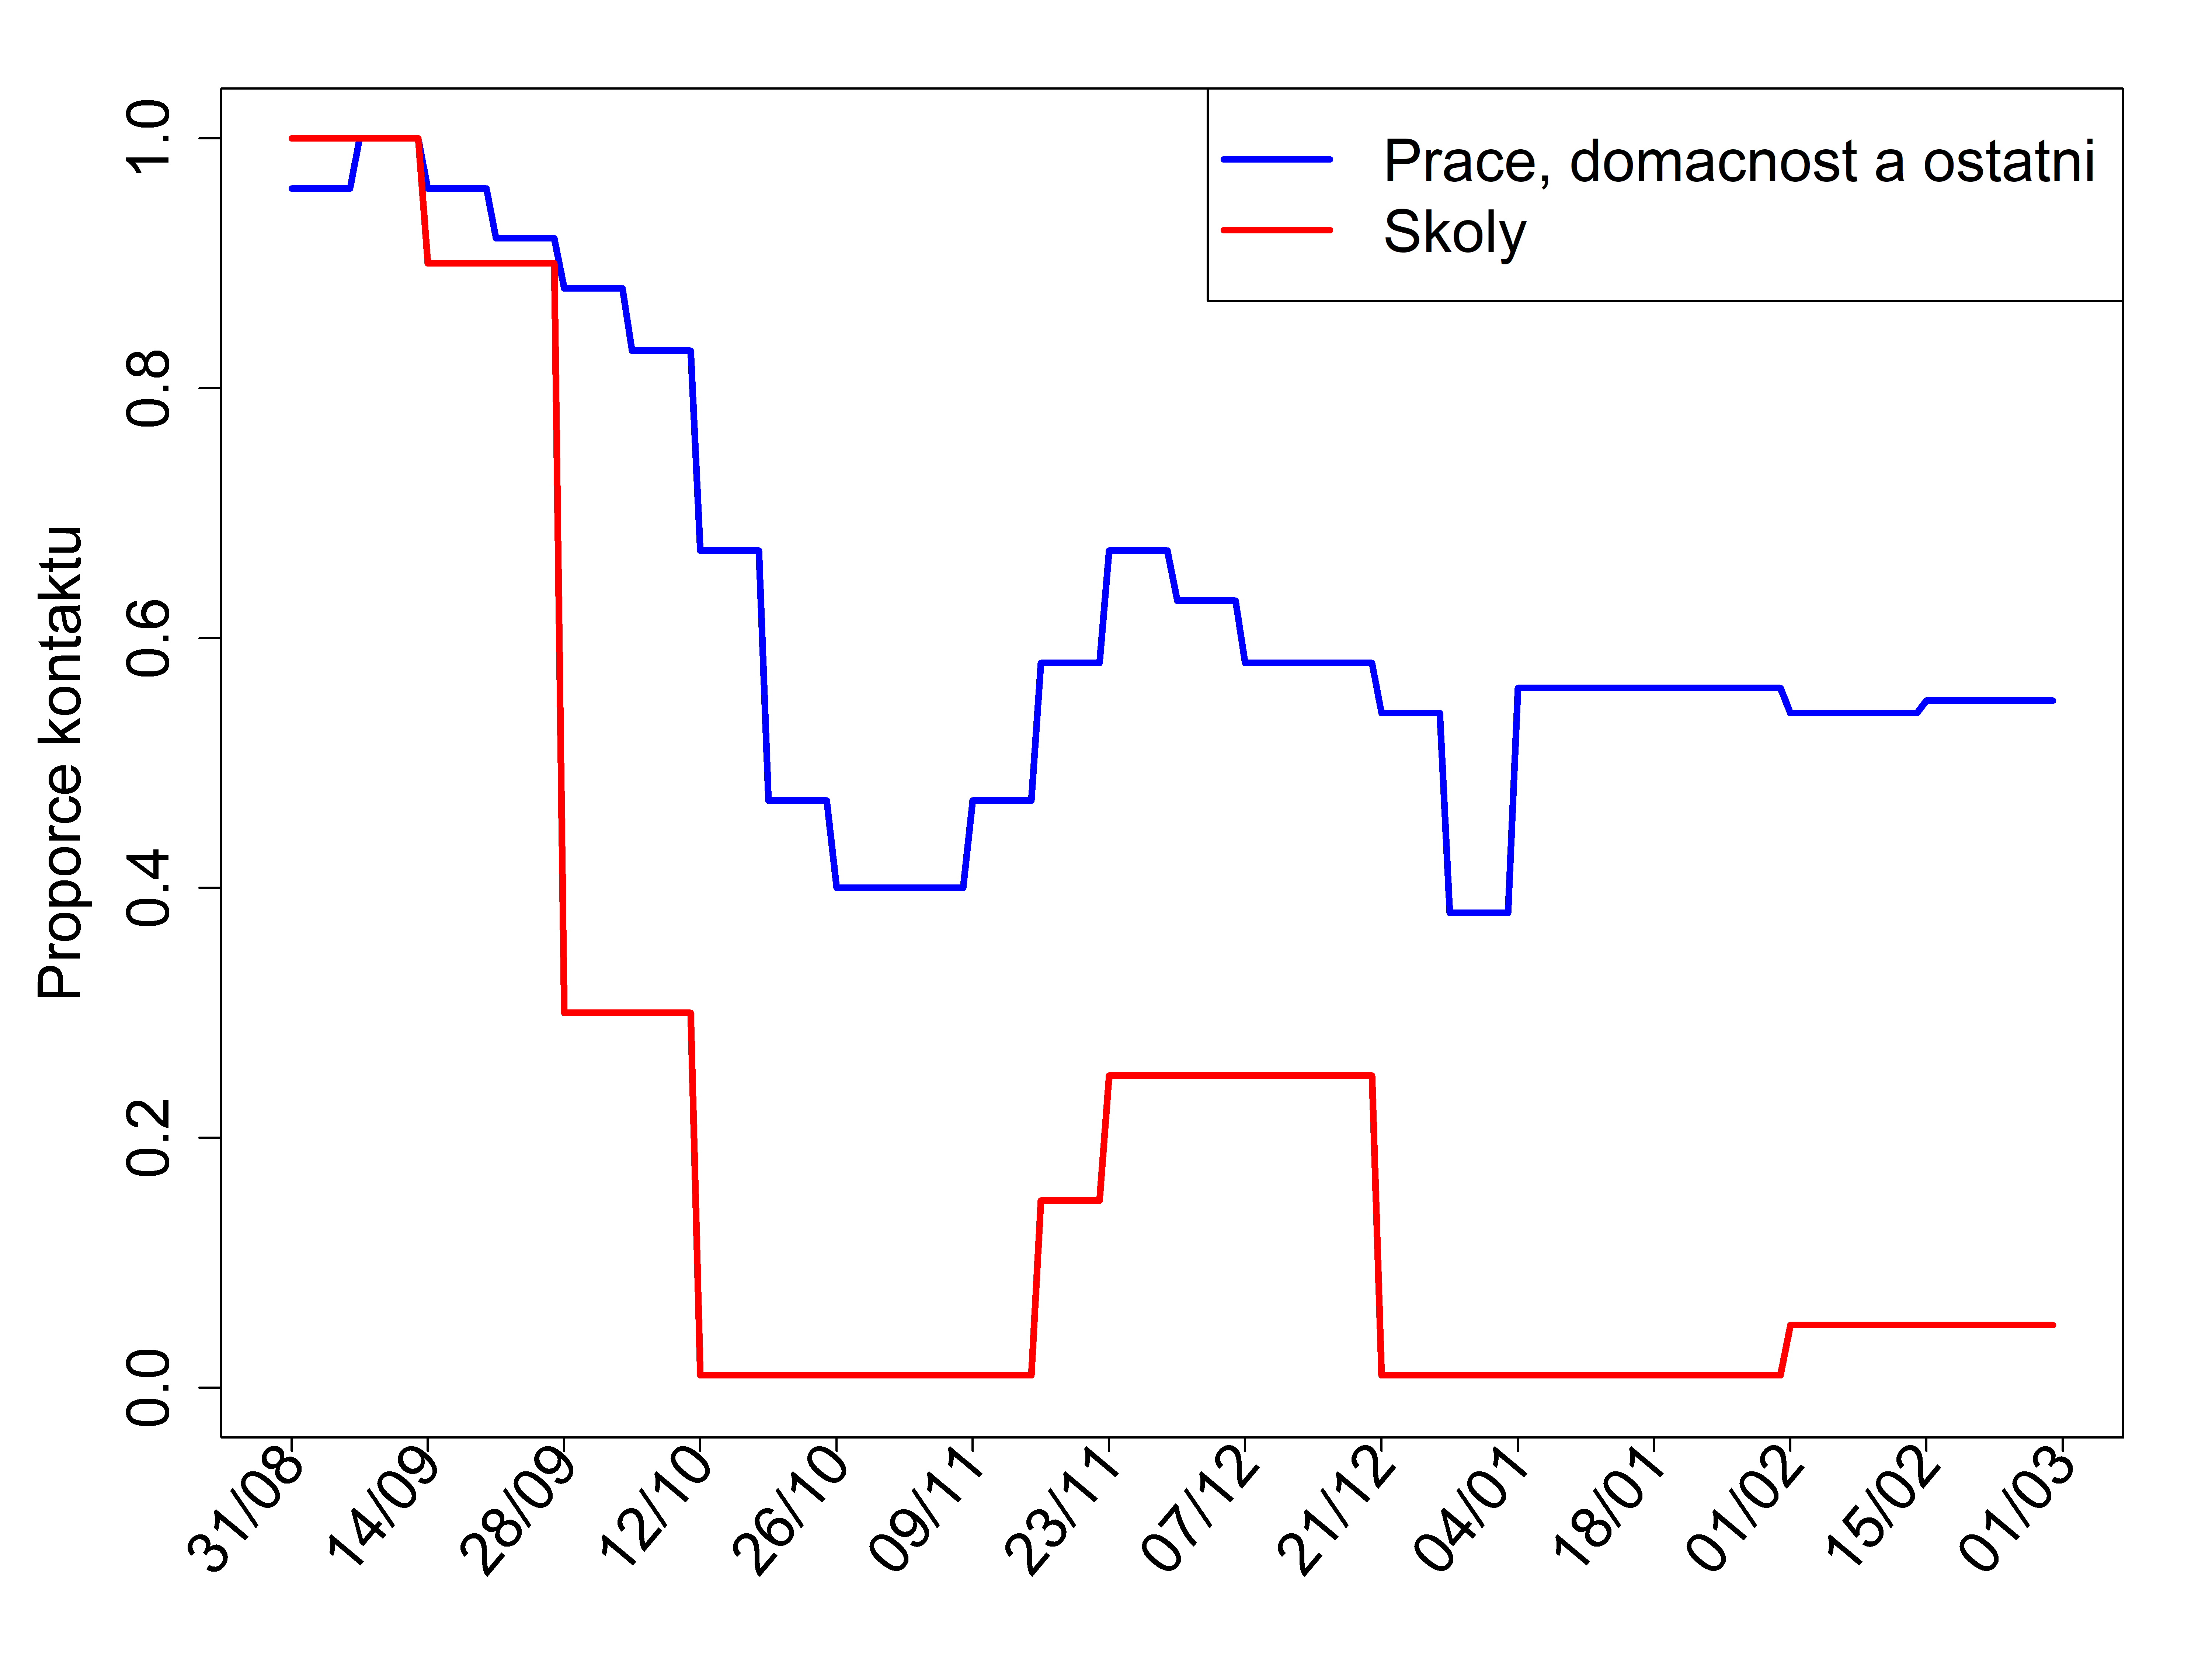
\includegraphics[width=\textwidth]{pic/figPAQ2.png}
		\end{minipage}
		\begin{minipage}[m]{0.45\linewidth}
			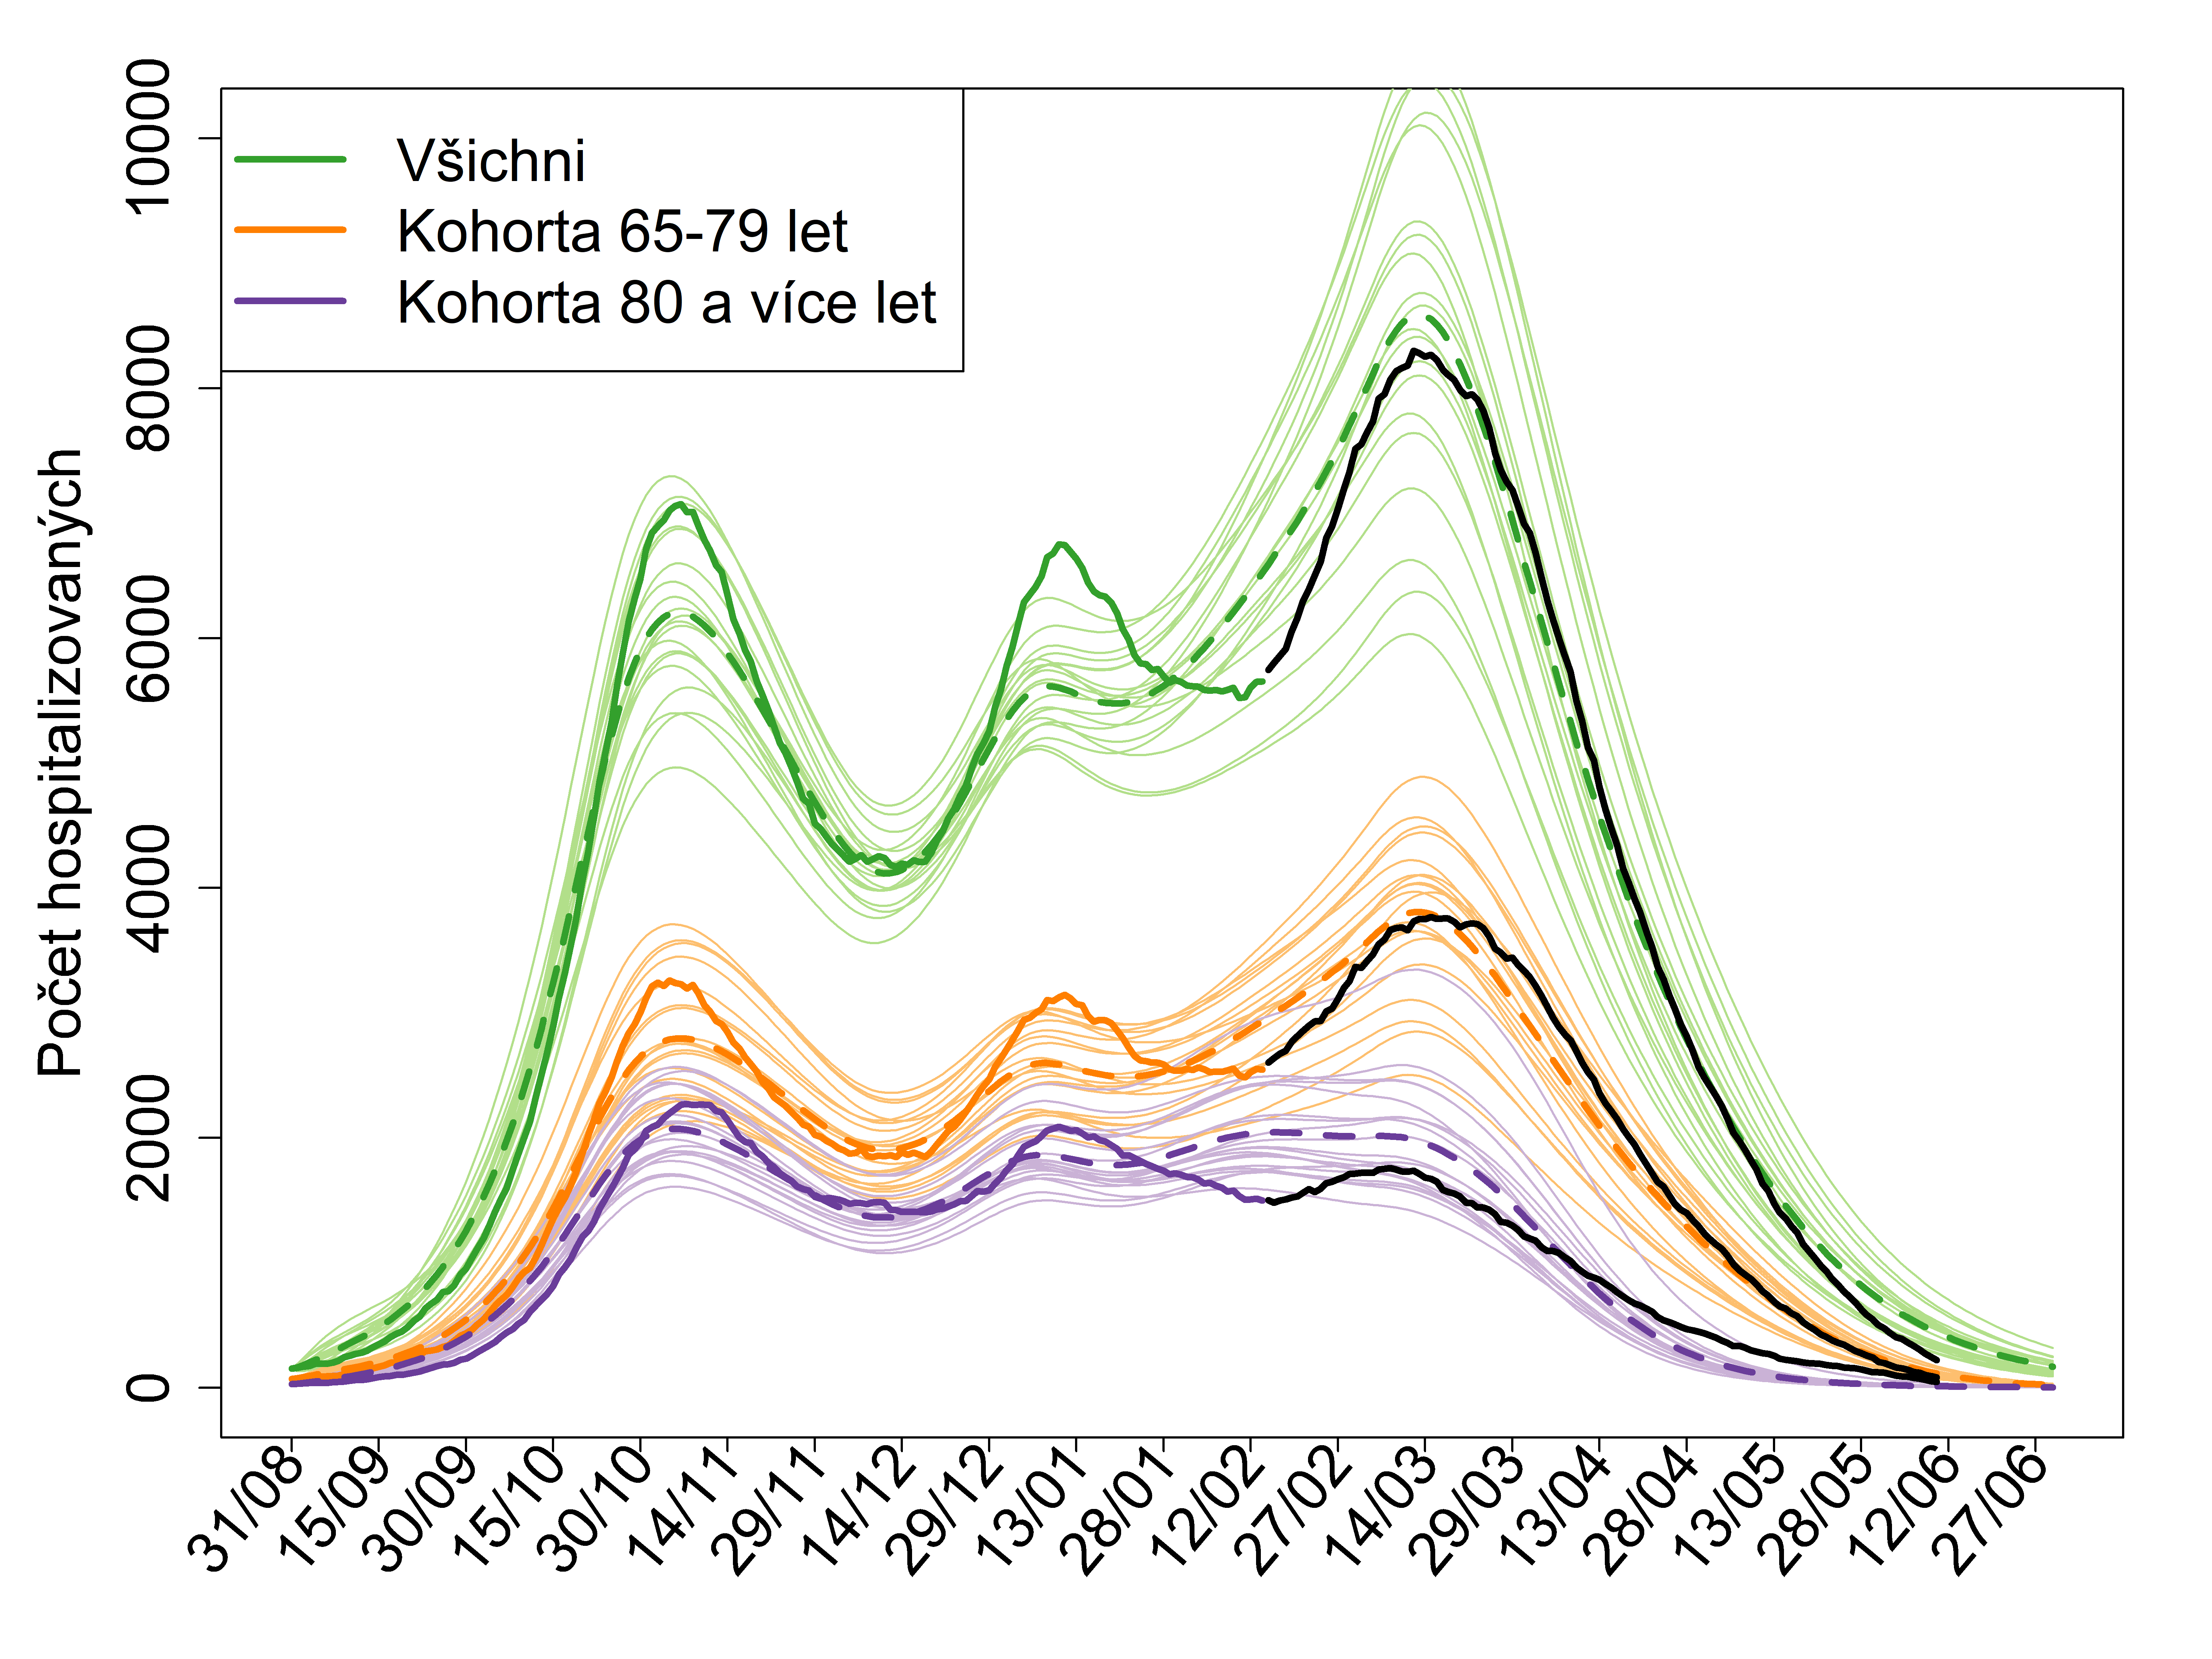
\includegraphics[width=\textwidth]{pic/vakcinace-hospital.png}
		\end{minipage} \\[1ex]
		\begin{minipage}[m]{0.45\linewidth}
			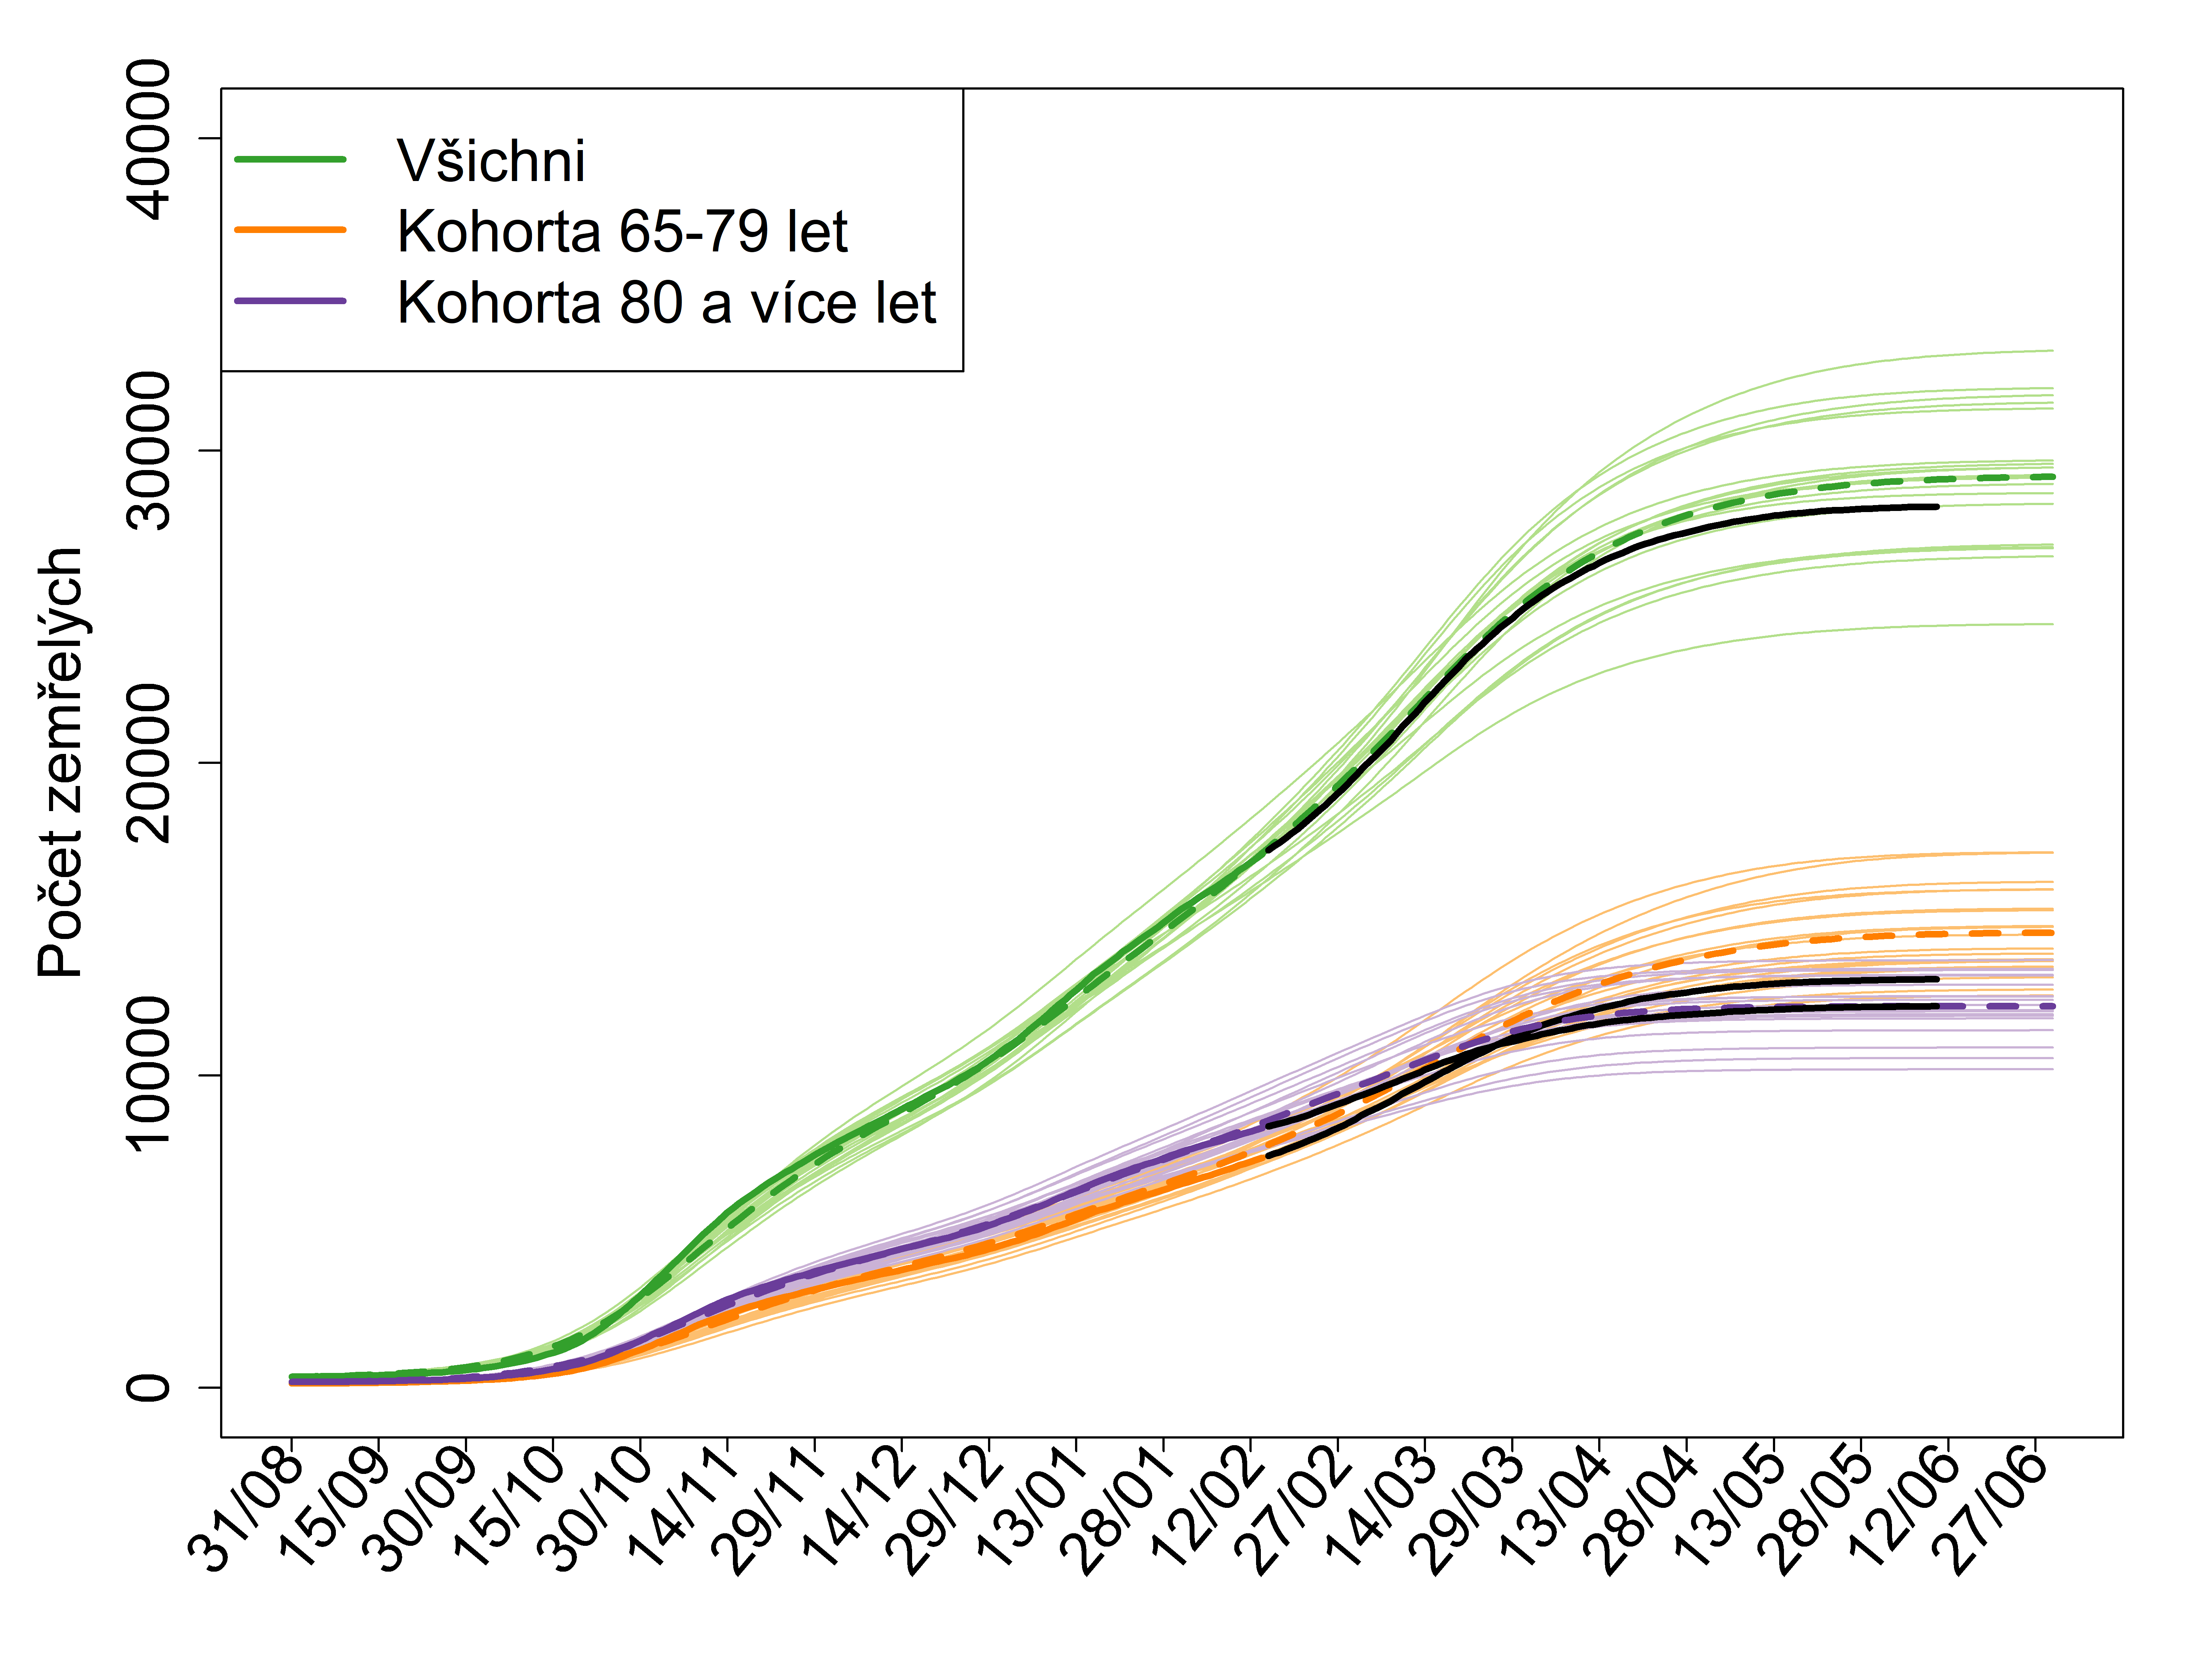
\includegraphics[width=\textwidth]{pic/vakcinace-death.png}
		\end{minipage} 
		\begin{minipage}[m]{0.45\linewidth}
			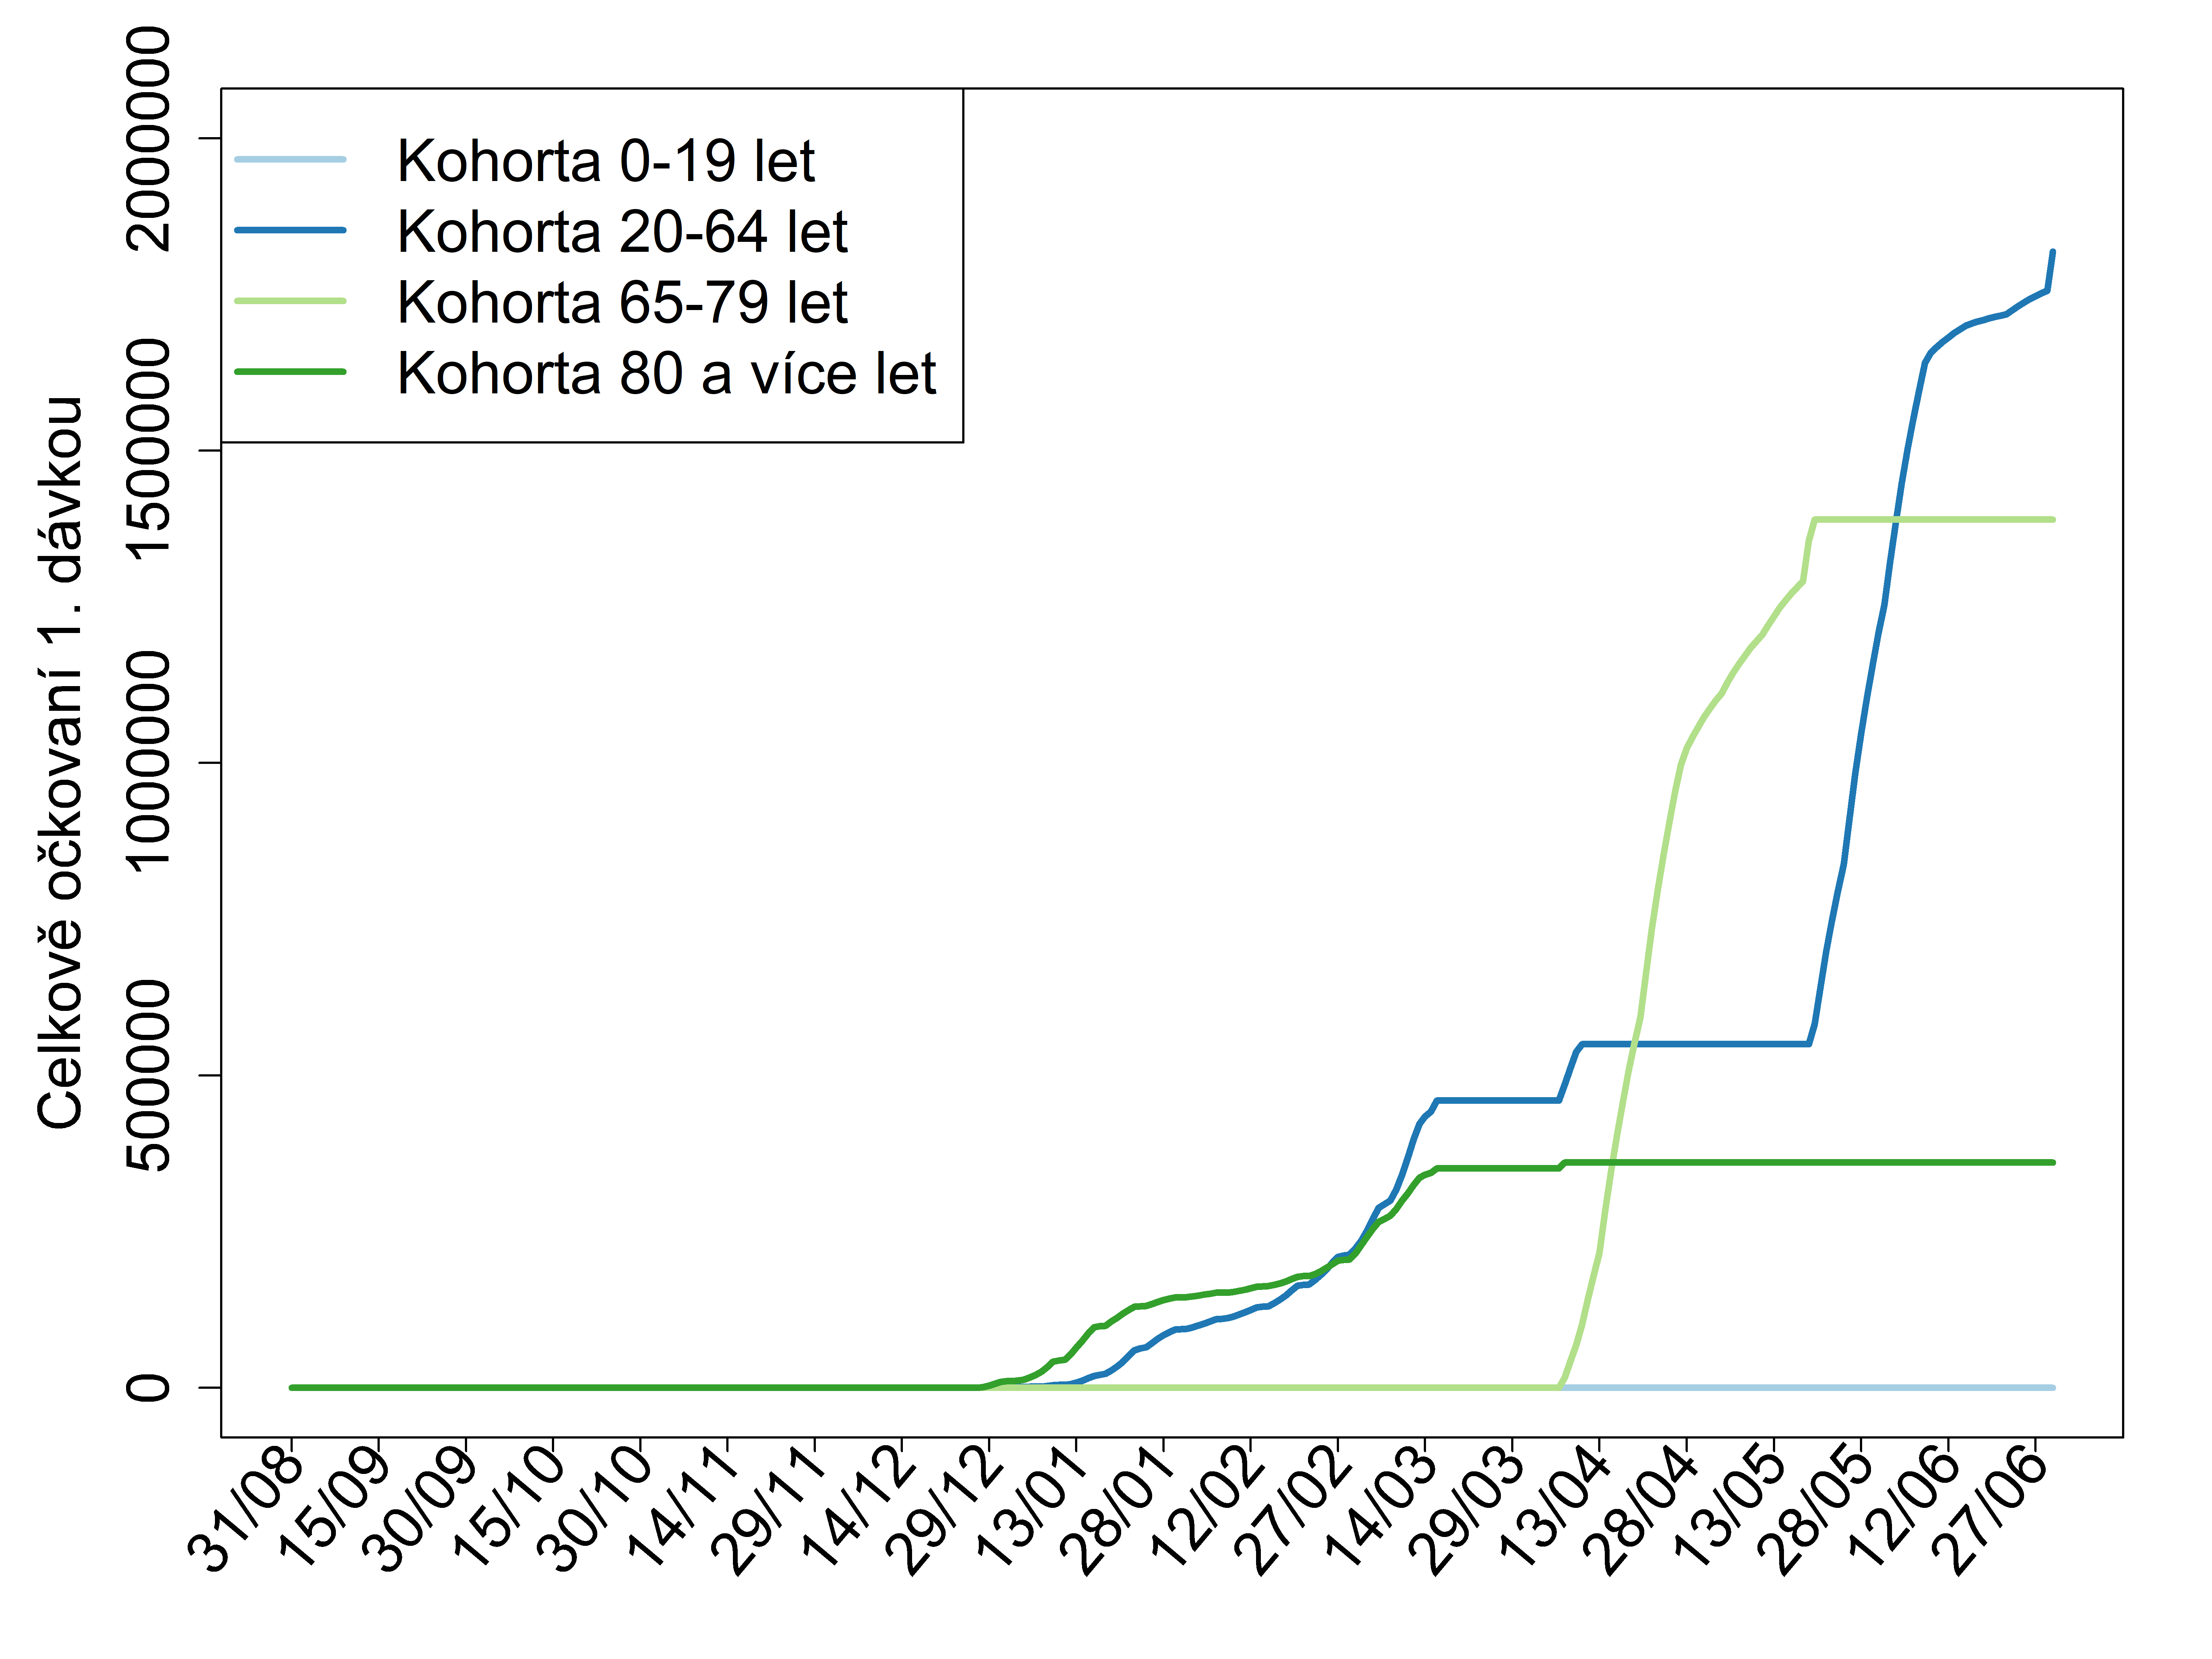
\includegraphics[width=\textwidth]{pic/vakcinace-davky.png}
		\end{minipage} 
	\end{center}
	\caption{Kalibrace modelu H, popisující dynamiku epidemie v celé České republice se zřetelem na dynamiku hospitalizací \cite{vaccpaper}. Horní levý panel: časový vývoj proporcionálního snížení kontaktů díky opatřením proti covid-19 v Česku \cite{paqcovid}; od 1.\ března 2021 jsou kontakty nastaveny na 45\,\% mimo školy a 1\,\% ve školách. Horní pravý a dolní levý panel: tenké křivky odpovídají 20 `nejlepším' světům ze 100000 simulovaných, vybraných metodou Approximate Bayesian Computation \cite{Toni_etal2009}, silné čárkované křivky jsou průměrné modelové trajektorie, silné plné křivky jsou pozorovaná data do 15.\ února 2021 použitá pro kalibraci, a nakonec černé křivky jsou pozorovaná data po tomto termínu naznačující dobré prediktivní možnosti modelu H. Dolní pravý panel: denní počty prvních dávek vakcín distribuované mezi jednotlivé věkové třídy při rozestupu mezi dávkami 21 dní.}
	\label{kalibraceH}
\end{figure}

\begin{figure}[h]
	\centering
	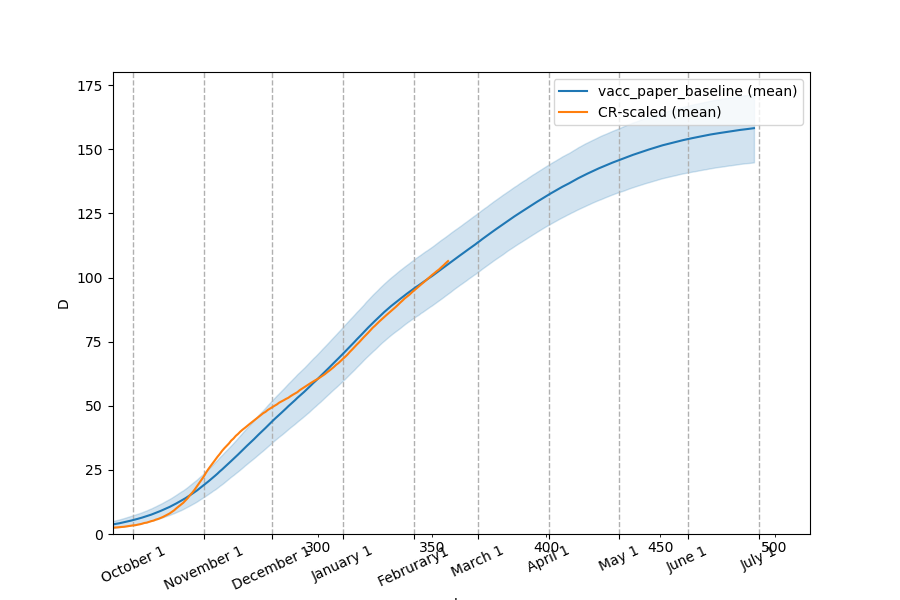
\includegraphics[width=0.6\textwidth]{pic/death_vacc_d.png}
	\caption{Kalibrace modelu M, popisujícího dynamiku epidemie ve středně velkém městě a okolí a inspirovaného Hodonínskou aglomerací \cite{M-techrep2021}. Graf ukazuje kumulativní počet zemřelých díky COVID-19 v modelových simulacích (modrá barva, střední hodnota $\pm$ standardní odchylka) ve srovnání se skutečnou situací v Česku škálovanou na použitou velikost populace v modelu M (oranžová barva).}
	\label{kalibraceM}
\end{figure}

Rozdíl mezi počtem zemřelých k 30.\ červnu mezi při rozestupu 42 dní a při rozestupu 21 dní, veličina, která nám slouží k posouzení potenciální výhodnosti odkladu druhé dávky o 42 dní místo původního rozestupu 21 dní, jistě závisí na řadě faktorů, včetně toho, jaké procesy vakcína ovlivňuje, s jakou účinností, jaká je rychlost dodávek vakcín či jakou intenzitu má epidemie. Ukážeme si výsledky několika scénářů, které s těmito faktory pracují; kompletní výsledky pak lze nalézt v práci \cite{vaccpaper}.

Povědomí o tom, jak vakcíny proti covid-19 fungují, se vyvíjelo postupně, jak se ve světě očkovalo čím dál více (nejvíce informací máme ze Spojeného království \cite{Hall_etal2021,Vasileiou_etal2021} a z Izraele \cite{Haas_etal2021}). První informace mluvily o vlivu na pravděpodobnost, že se u nakaženého jedince objeví symptomy a na pravděpodobnost přenosu infekce z infekčního na vnímavého jedince. Poslední studie pak hovoří o vlivu na všechny procesy v infekčním řetězci: kromě už zmíněných dvou také na pravděpodobnost hospitalizace, vážného stavu a úmrtí \cite{Haas_etal2021}. Známé už jsou také první odhady účinnosti proti novým nakažlivějším variantám viru SARS-CoV-2 \cite[a reference uvnitř]{Shapiro_etal2021,delta}. 

Všechny tři námi použité modely mohou snadno zahrnout vliv vakcín na pravděpodobnost toho, že se u nakaženého jedince objeví symptomy a na pravděpodobnost přenosu infekce z infekčního na vnímavého jedince. Výsledky pro tyto scénáře shrnuje obr.\,\ref{figvacc1}, předpokládající skutečnou intenzitu epidemie a realistické dodávky vakcín (odhadnuté k 16.\ 3.\ 2021) v Česku. Tento i další obrázky \ref{figvacc2} a \ref{figvacc3} mají jednotnou strukturu: pro zvolený scénář (jak vakcína funguje, intenzita epidemie, rychlost dodávek vakcín) uvažujeme všechny možné kombinace účinnosti vakcíny po první a druhé dávce (účinnost 7 dní po druhé dávce je vždy nejméně taková jako účinnost 14 dní po dávce první). Výhodnost rozestupu mezi dávkami 21 dní je vyznačena odstíny modré (kladné hodnoty, více zemřelých pro rozestup 42 dní), kdežto výhodnost odkladu o 42 dní je vyznačena odstíny červené (záporné hodnoty, více zemřelých pro rozestup 21 dní). Obrázek \ref{figvacc1} ukazuje, že delší rozestup 42 dní je ve všech uvedených scénářích výhodnější jen pokud účinnost po druhé dávce není o mnoho vyšší než po dávce první, přičemž množství kombinací účinnosti první a druhé dávky, pro které je odklad o 42 dní výhodnější, je největší v případě vlivu vakcíny na pravděpodobnost, že se u nakaženého jedince objeví symptomy.

\begin{figure}[h]
	\begin{center}
		\begin{minipage}[m]{0.3\linewidth}
			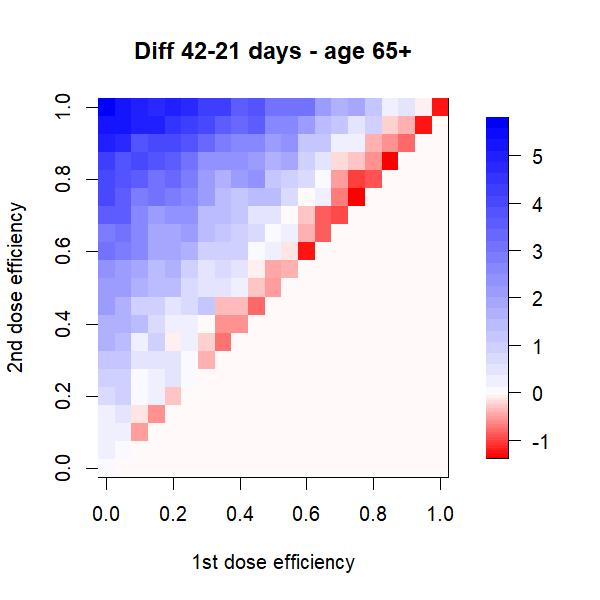
\includegraphics[width=\textwidth]{pic/SP_DIFF_mean_T.jpg}
		\end{minipage}
		\begin{minipage}[m]{0.3\linewidth}
			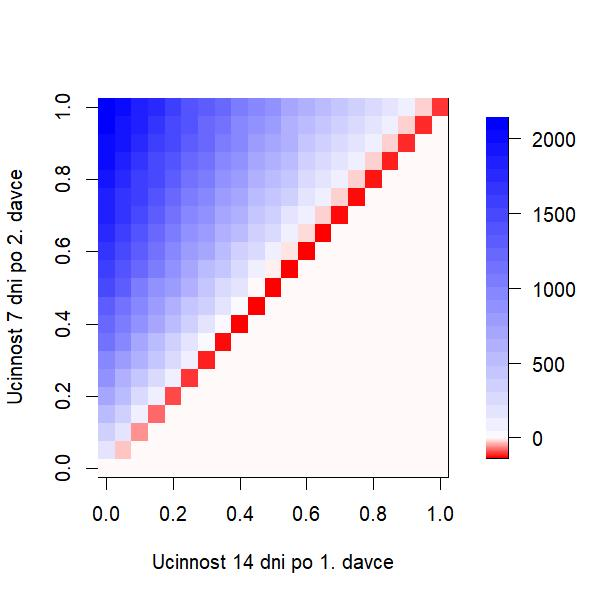
\includegraphics[width=\textwidth]{pic/SL_DIFF_mean_T.jpg}
		\end{minipage}
		\begin{minipage}[m]{0.3\linewidth}
			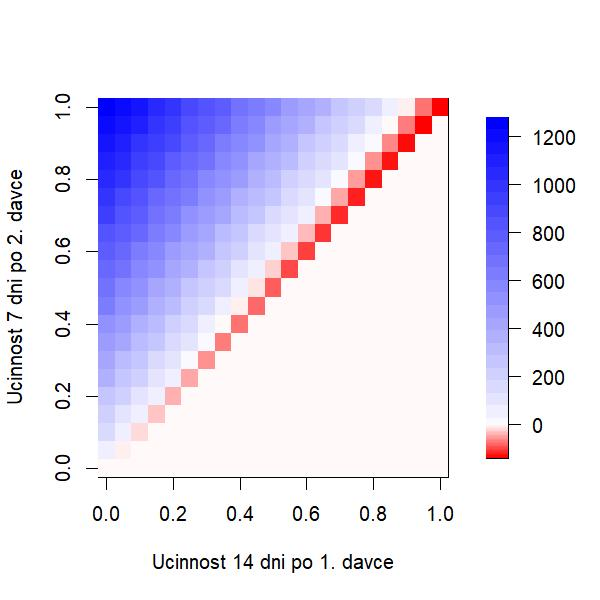
\includegraphics[width=\textwidth]{pic/SM_DIFF_mean_T.jpg}
		\end{minipage} \\[1ex]
		\begin{minipage}[m]{0.3\linewidth}
			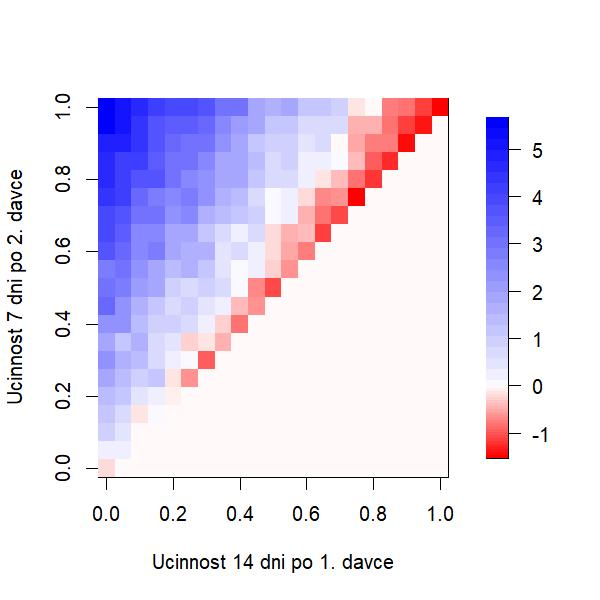
\includegraphics[width=\textwidth]{pic/AP_DIFF_mean_T.jpg}
		\end{minipage}
		\begin{minipage}[m]{0.3\linewidth}
			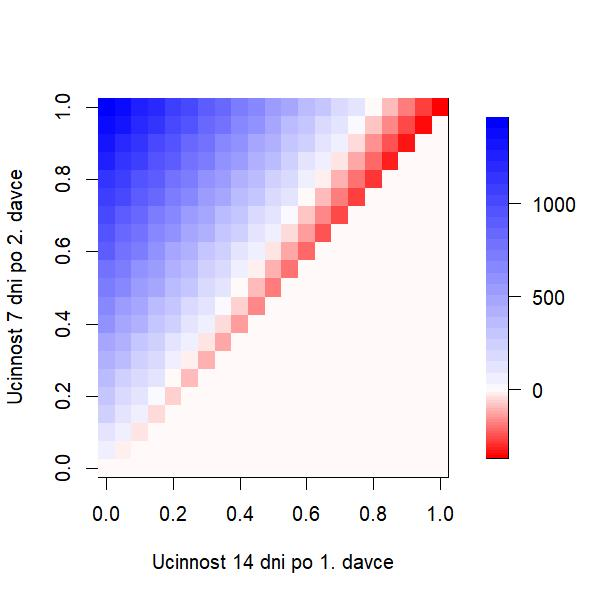
\includegraphics[width=\textwidth]{pic/AL_DIFF_mean_T.jpg}
		\end{minipage}
		\begin{minipage}[m]{0.3\linewidth}
			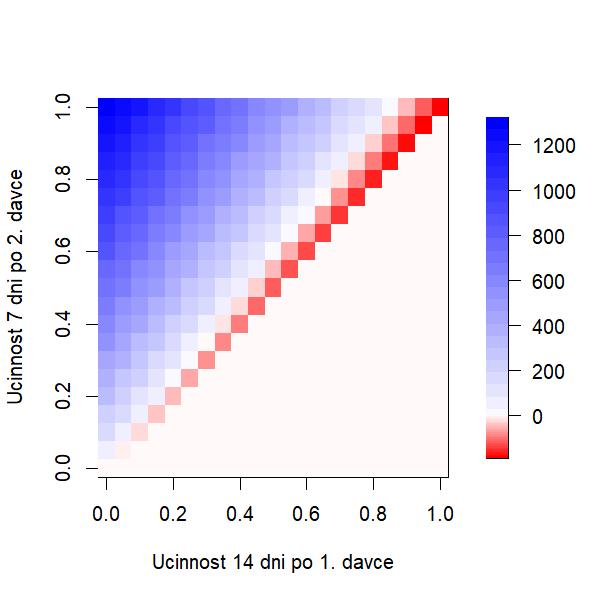
\includegraphics[width=\textwidth]{pic/AM_DIFF_mean_T.jpg}
		\end{minipage} \\[1ex]
		\begin{minipage}[m]{0.3\linewidth}
			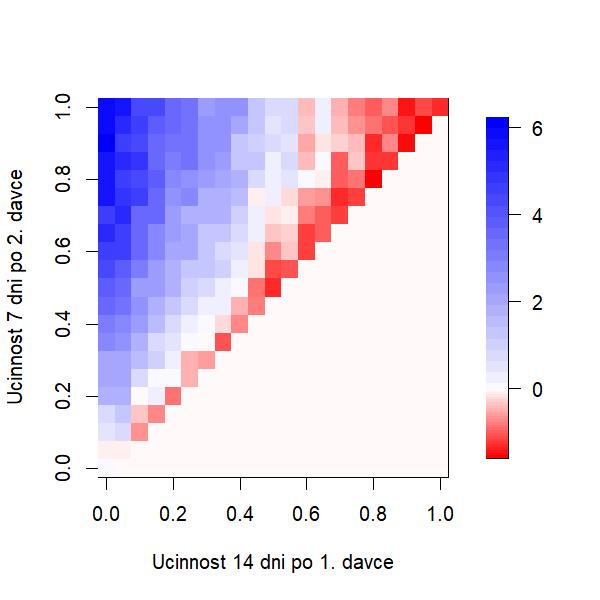
\includegraphics[width=\textwidth]{pic/SAP_DIFF_mean_T.jpg}
		\end{minipage}
		\begin{minipage}[m]{0.3\linewidth}
			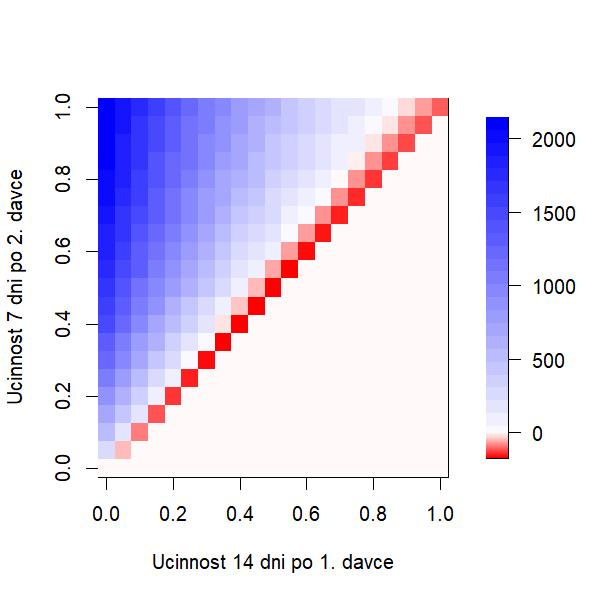
\includegraphics[width=\textwidth]{pic/SAL_DIFF_mean_T.jpg}
		\end{minipage}
		\begin{minipage}[m]{0.3\linewidth}
			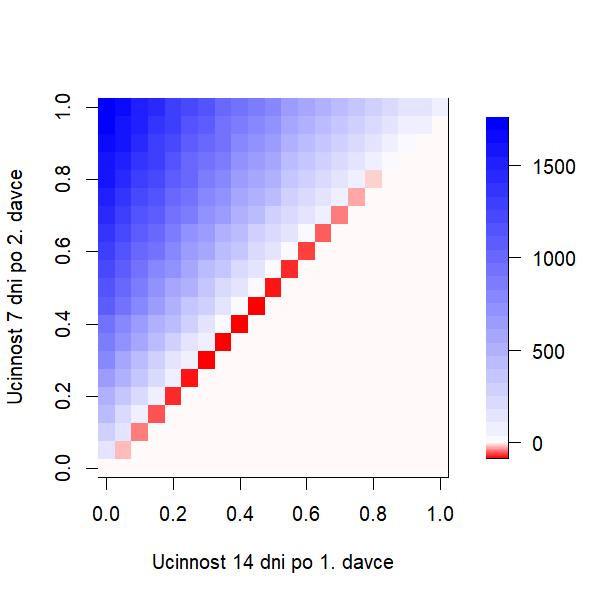
\includegraphics[width=\textwidth]{pic/SAM_DIFF_mean_T.jpg}
		\end{minipage}
	\end{center}
	\caption{Výhodnost odkladu druhé dávky vakcíny o tři týdny z původních 21 na 42 dní pro několik typů fungování vakcíny, jak ji předpovídají naše tři modely. Horní řádek: efekt vakcíny na pravděpodobnost přenosu infekce z infekčního na vnímavého jedince, střední řádek: efekt vakcíny na pravděpodobnost, že se u nakaženého jedince objeví symptomy, dolní řádek: kombinace obou těchto typů fungování vakcíny. Levý sloupec: model M, střední sloupec: model H, pravý sloupec: model F.}
	\label{figvacc1}
\end{figure}
 
Obr.\,\ref{figvacc2} shrnuje modelové predikce pro případy, kdy vakcína ovlivňuje postupně pravděpodobnost vážného stavu, úmrtí a kombinace vážného stavu a úmrtí. Množství kombinací účinnosti první a druhé dávky, pro které je rozestup 42 dní výhodnější, postupně roste.
 
\begin{figure}[h]
	\begin{center}
		\begin{minipage}[m]{0.3\linewidth}
			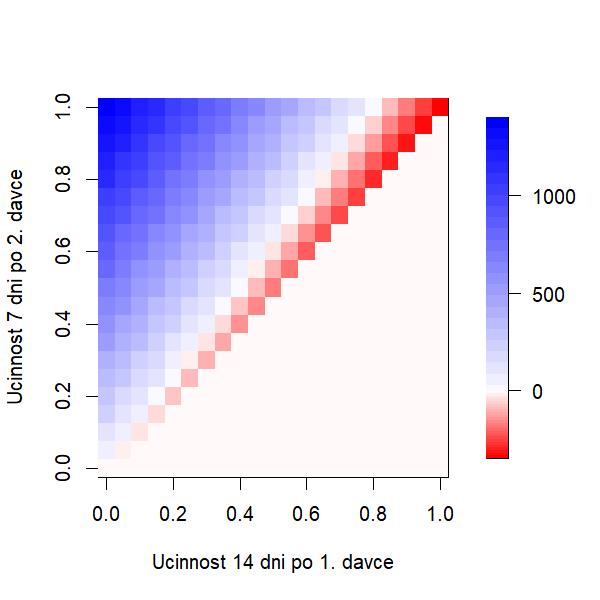
\includegraphics[width=\textwidth]{pic/JL_DIFF_mean_T.jpg}
		\end{minipage}
		\begin{minipage}[m]{0.3\linewidth}
			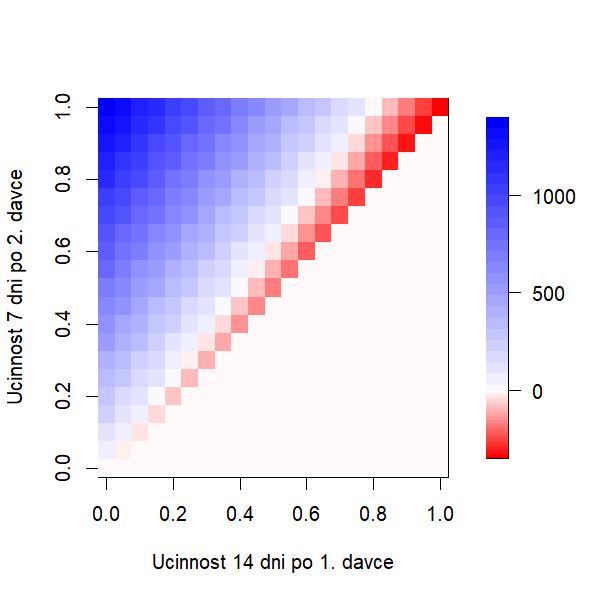
\includegraphics[width=\textwidth]{pic/DL_DIFF_mean_T.jpg}
		\end{minipage}
		\begin{minipage}[m]{0.3\linewidth}
			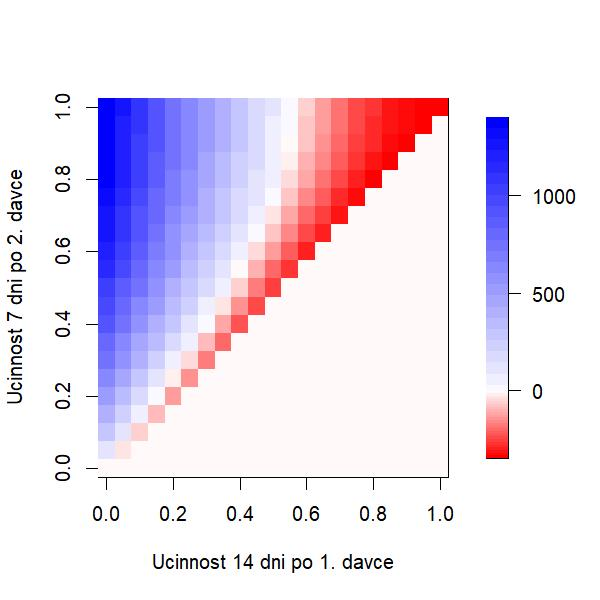
\includegraphics[width=\textwidth]{pic/JDL_DIFF_mean_T.jpg}
		\end{minipage}
	\end{center}
	\caption{Výhodnost odkladu druhé dávky vakcíny o tři týdny z původních 21 na 42 dní pro několik dalších možných typů fungování vakcíny (výsledky modelu H). Levý panel: efekt vakcíny na pravděpodobnost vážného stavu při hospitalizaci, střední panel: efekt vakcíny na pravděpodobnost úmrtí při hospitalizaci, pravý panel: kombinace obou těchto typů fungování vakcíny.}
	\label{figvacc2}
\end{figure}

V řadě zemí bohužel není tak nízká intenzita epidemie ani takové dodávky vakcín jako v Česku. Modelové výstupy naznačují, že množství kombinací účinnosti první a druhé dávky, pro které je rozestup 42 dní výhodnější, roste s rostoucí intenzitou epidemie a s klesající rychlostí dodávek vakcín (obr.\,\ref{figvacc3}). Pro tento obrázek předpokládáme vliv vakcíny na pravděpodobnost, že se u nakaženého jedince objeví symptomy a na pravděpodobnost přenosu infekce z infekčního na vnímavého jedince, avšak kvalitativně analogické výsledky vycházejí i pro jiné předpoklady o fungování vakcíny. Přestože vliv intenzity epidemie je nezanedbatelný, mnohem větší je vliv rychlosti vakcinace, kdy v zásadě bez ohledu na způsob fungování vakcíny je rozestup mezi dávkami 42 dní výhodný pro všechny rozumné kombinace účinností první a druhé dávky.

\begin{figure}[h]
	\begin{center}
		\begin{minipage}[m]{0.3\linewidth}
			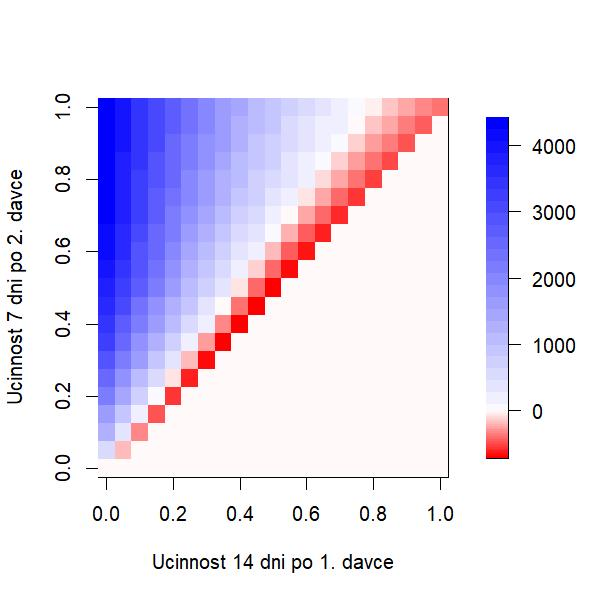
\includegraphics[width=\textwidth]{pic/SA65L_DIFF_mean_T.jpg}
		\end{minipage}
		\begin{minipage}[m]{0.3\linewidth}
			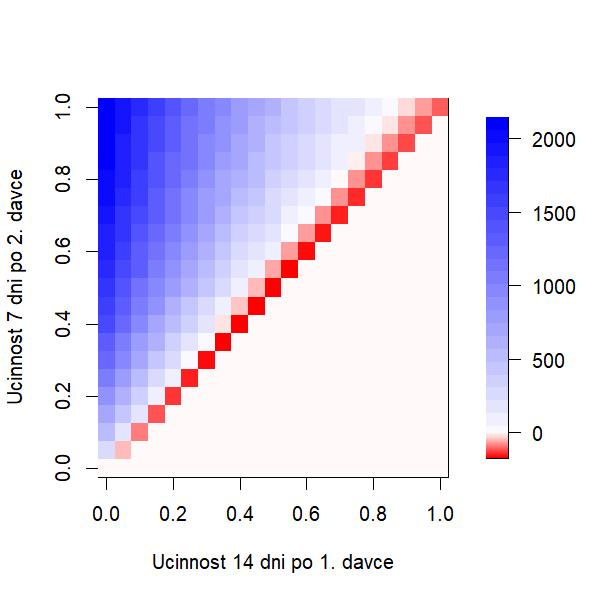
\includegraphics[width=\textwidth]{pic/SAL_DIFF_mean_T.jpg}
		\end{minipage}
		\begin{minipage}[m]{0.3\linewidth}
			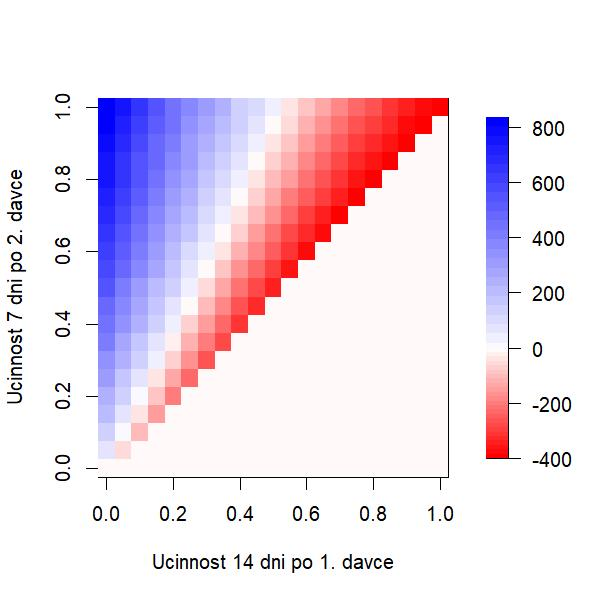
\includegraphics[width=\textwidth]{pic/SA4lessL_DIFF_mean_T.jpg}
		\end{minipage}
	\end{center}
	\caption{Výhodnost odkladu druhé dávky vakcíny o tři týdny z původních 21 na 42 dní za předpokladu vlivu vakcíny na pravděpodobnost, že se u nakaženého jedince objeví symptomy a na pravděpodobnost přenosu infekce z infekčního na vnímavého jedince, pro různé další specifické scénáře. Levý panel: intenzivnější epidemie, kontakty zvýšeny ze 45\,\% na 65\,\%, střední panel: intenzita epidemie a rychlost očkování jako v Česku, pravý panel: nízká rychlost očkování, snížená na čtvrtinu ve srovnání s Českem.}
	\label{figvacc3}
\end{figure}

\section*{Závěr}

V této kapitole jsme se pokusili ukázat, že stejně jako při zkoumání mnoha jiných aspektů šíření infekčních nemocí hraje i při tvorbě strategií očkování matematické modelování nezastupitelnou roli. Zásadním konceptem, který modely do epidemiologie vnesly, je práh kolektivní imunity. Už McKendrick s Kermackem v rámci svého SIR modelu vysvětlili, proč epidemie odezní dříve, než patogen stačí nakazit všechny jedince ve společnosti \cite[viz také kapitola \ref{Typy_modelu}]{Bacaer2011}. Se zvyšujícím se podílem imunizovaných jedinců v populaci totiž klesá podíl kontaktů mezi infekčními a vnímavými jedinci, a od určitého okamžiku tak rychlost, s níž přibývají nové případy bude nižší než rychlost, s jakou se stávající infekční jedinci uzdravují. Protože vakcinace je jen jiná forma imunizace, byl jen krok k tomu, dovodit význam tohoto závěru pro vakcinaci: naočkujeme-li dostatečnou část společnosti, zabráníme dalšímu systematickému nárůstu nových případů. A právě kritická hodnota podílu imunizovaných jedinců, za kterou toto nastane, se nazývá práh kolektivní imunity.

Práh kolektivní imunity však nebudeme v důsledku nejistoty bytostně spojené s modelováním nikdy znát přesně. Navíc ani v případě jeho případného dosažení nemůžeme vyloučit objevení se lokálních ohnisek, neboť imunizovaná část společnosti zcela jistě není nikdy v rámci populace rovnoměrně rozložená. Jakkoli vypočtený práh kolektivní imunity je tak třeba brát spíše jako jakýsi indikátor toho, jak daleko od něj se nacházíme a jaký vliv tento rozdíl na další šíření epidemie může mít. 

Matematické modelování epidemií výrazně přispělo k hledání odpovědi na otázku, jaké skupiny společnosti prioritně očkovat \cite{Bubar_etal2021,Moore_etal2021b}. Závěry těchto a dalších studií tohoto typu vedly k zavedení strategie očkování od nejstarších věkových skupin k postupně mladším ročníkům. V této kapitole jsme si představili aplikaci několika modelů epidemie covid-19 vyvinutých v rámci centra BISOP na zkoumání jiné otázky, totiž otázky výhodnosti odkladu druhé dávky vakcíny o 42 dní ve srovnání s původními 21 dny doporučenými výrobcem (jako příklad jsme si zvolili vakcínu Comirnaty společností Pfizer a BioNTech). Výsledky modelové studie naznačují, že rozestup mezi dávkami v délce 42 dní je nejvýhodnější v situacích, kdy vakcinace snižuje pravděpodobnost výskytu těžkého stavu či pravděpodobnost úmrtí, epidemie je relativně intenzivní a rychlost očkování je nízká, kdežto původní rozestup 21 dní je výhodnější, když vakcinace ovlivňuje pravděpodobnost, že se nakazíme při kontaktu s nemocným či pravděpodobnost objevení se symptomů, epidemie není příliš intenzivní a rychlost očkování je relativně vysoká. Výzvou pro vývojáře stále složitějších matematických modelů, tak zůstává schopnost dobře tyto modely a jejich předpovědi vysvětlit jejich možným odběratelům, tvůrcům veřejných politik, a dosáhnout tak vzájemné důvěry nezbytné pro řešení jakékoli epidemie \cite{BasuAndrews2013}.